\chapter{Podręcznik użytkownika (Karolina Makuch)}
\par W celu wytłumaczenia obsługi stworzonej aplikacji oraz zaprezentowaniu jej wizualnej strony przygotowano podręcznik użytkownika. Zawiera on poszczególne etapy wykonywania najważniejszych funkcjonalności.
Aplikacja została zaimplementowana w dwóch wersjach językowych. Dostępny jest język polski oraz angielski.
W trakcie implementacji została podjęta decyzja o zmianie wyglądu aplikacji. Zdecydowano się na weselsze kolory.

\begin{figure}[h]

\centering
\null\hfill
\subfloat[Widok logowania.\label{fig:firstDesign1}]{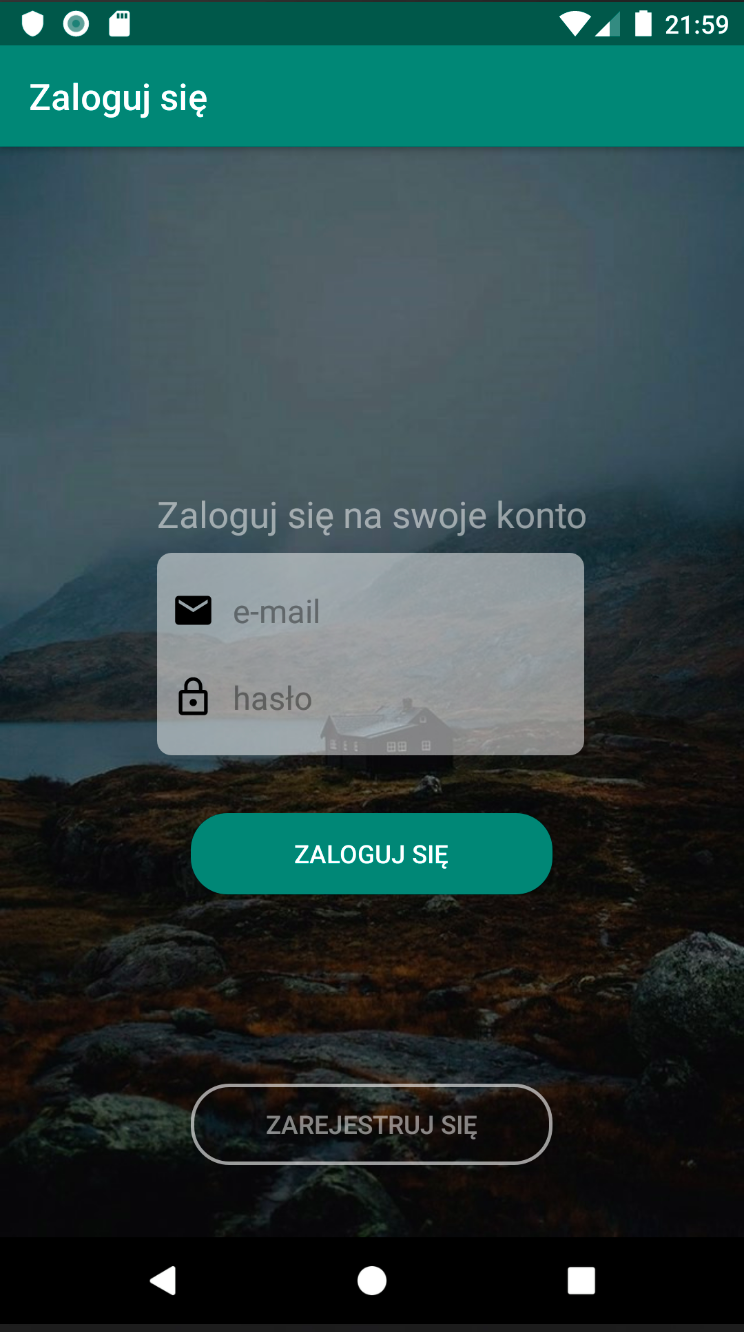
\includegraphics[width=0.32\textwidth]{firstDesign1}}
\hfill
\subfloat[Widok podróży.\label{fig:firstDesign2}]{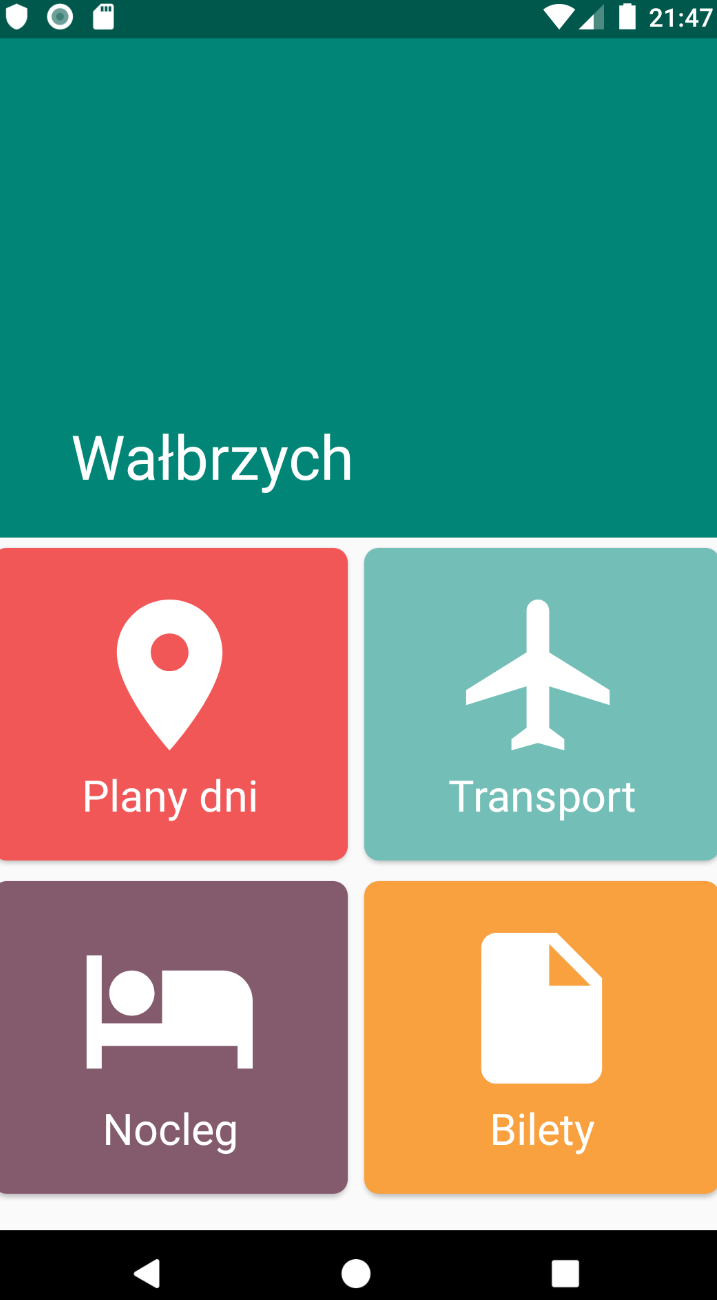
\includegraphics[width=0.32\textwidth]{firstDesign2}}
\hfill
\subfloat[Plan podróży.\label{fig:firstDesign3}]{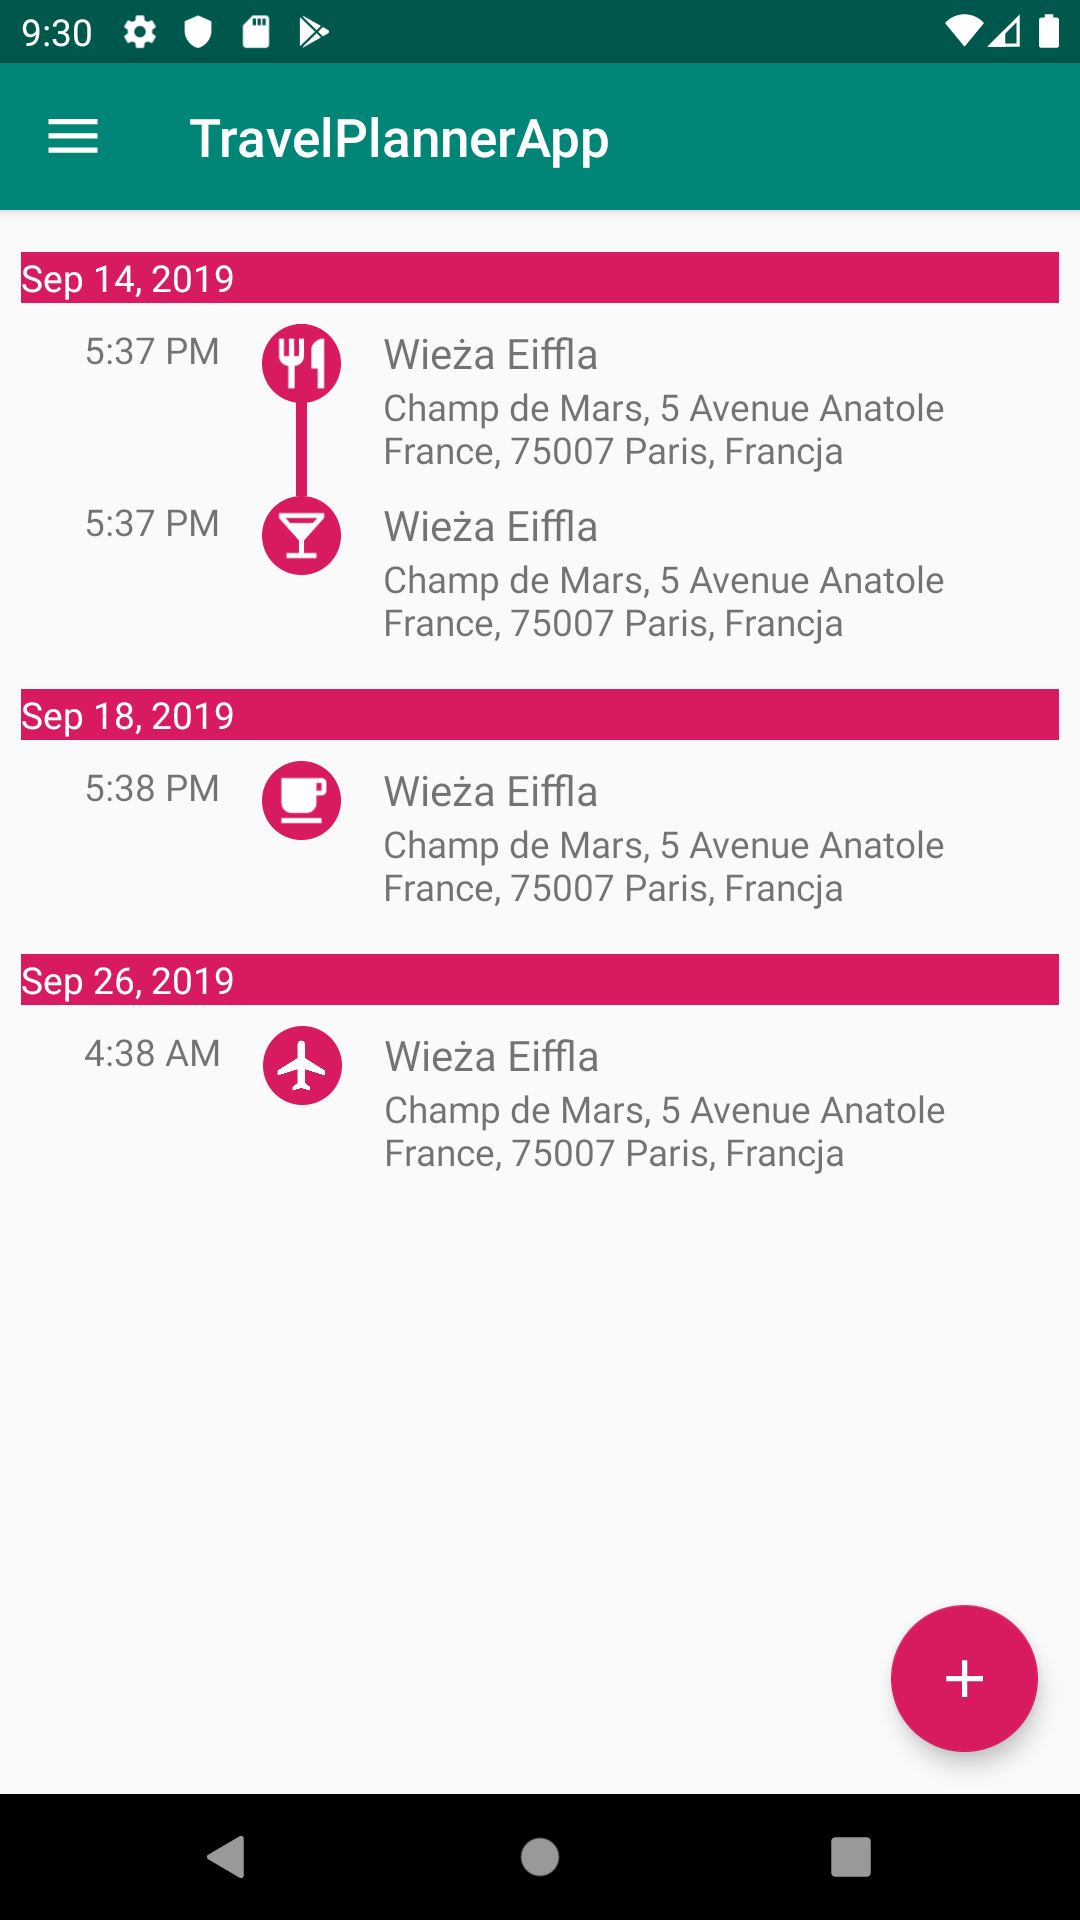
\includegraphics[width=0.32\textwidth]{firstDesign3}}
\hfill\null

\caption{Pierwszy projekt interfejsu użytkownika.}
\label{fig:podrecznik10}
\end{figure}
\FloatBarrier

\section{Rejestracja oraz logowanie użytkownika}
Użytkownik pierwszy raz uruchamiający aplikację i chcący z niej korzystać powinien stworzyć własne konto. W tym celu należy:

\begin{enumerate}
\item Kliknąć przycisk \textit{Zarejestruj się}.
\item W widoku rejestracji (rys. 10.2a) podać swój adres mailowy oraz hasło spełniające wymagania:
\begin{itemize}
\item przynajmniej 8 znaków długości,
\item przynajmniej jedna cyfra,
\item przynajmniej jedna duża litera,
\item przynajmniej jedna mała litera.
\end{itemize}

\item Kliknąć \textit{Zarejestruj się}.
\item Po pojawieniu się powiadomienia \textit{Twoje konto zostało utworzone} następuje automatyczne przekierowanie do widoku logowania (rys. 10.2b).
\item Uzupełnić pola widoku logowania tymi samymi danymi.
\item Logowanie następuje w momencie uzupełnienia danych oraz kliknięcia \textit{Zaloguj się}.
\end{enumerate}

\begin{figure}[h]

\centering
\null\hfill
\subfloat[Widok logowania.\label{fig:loginView}]{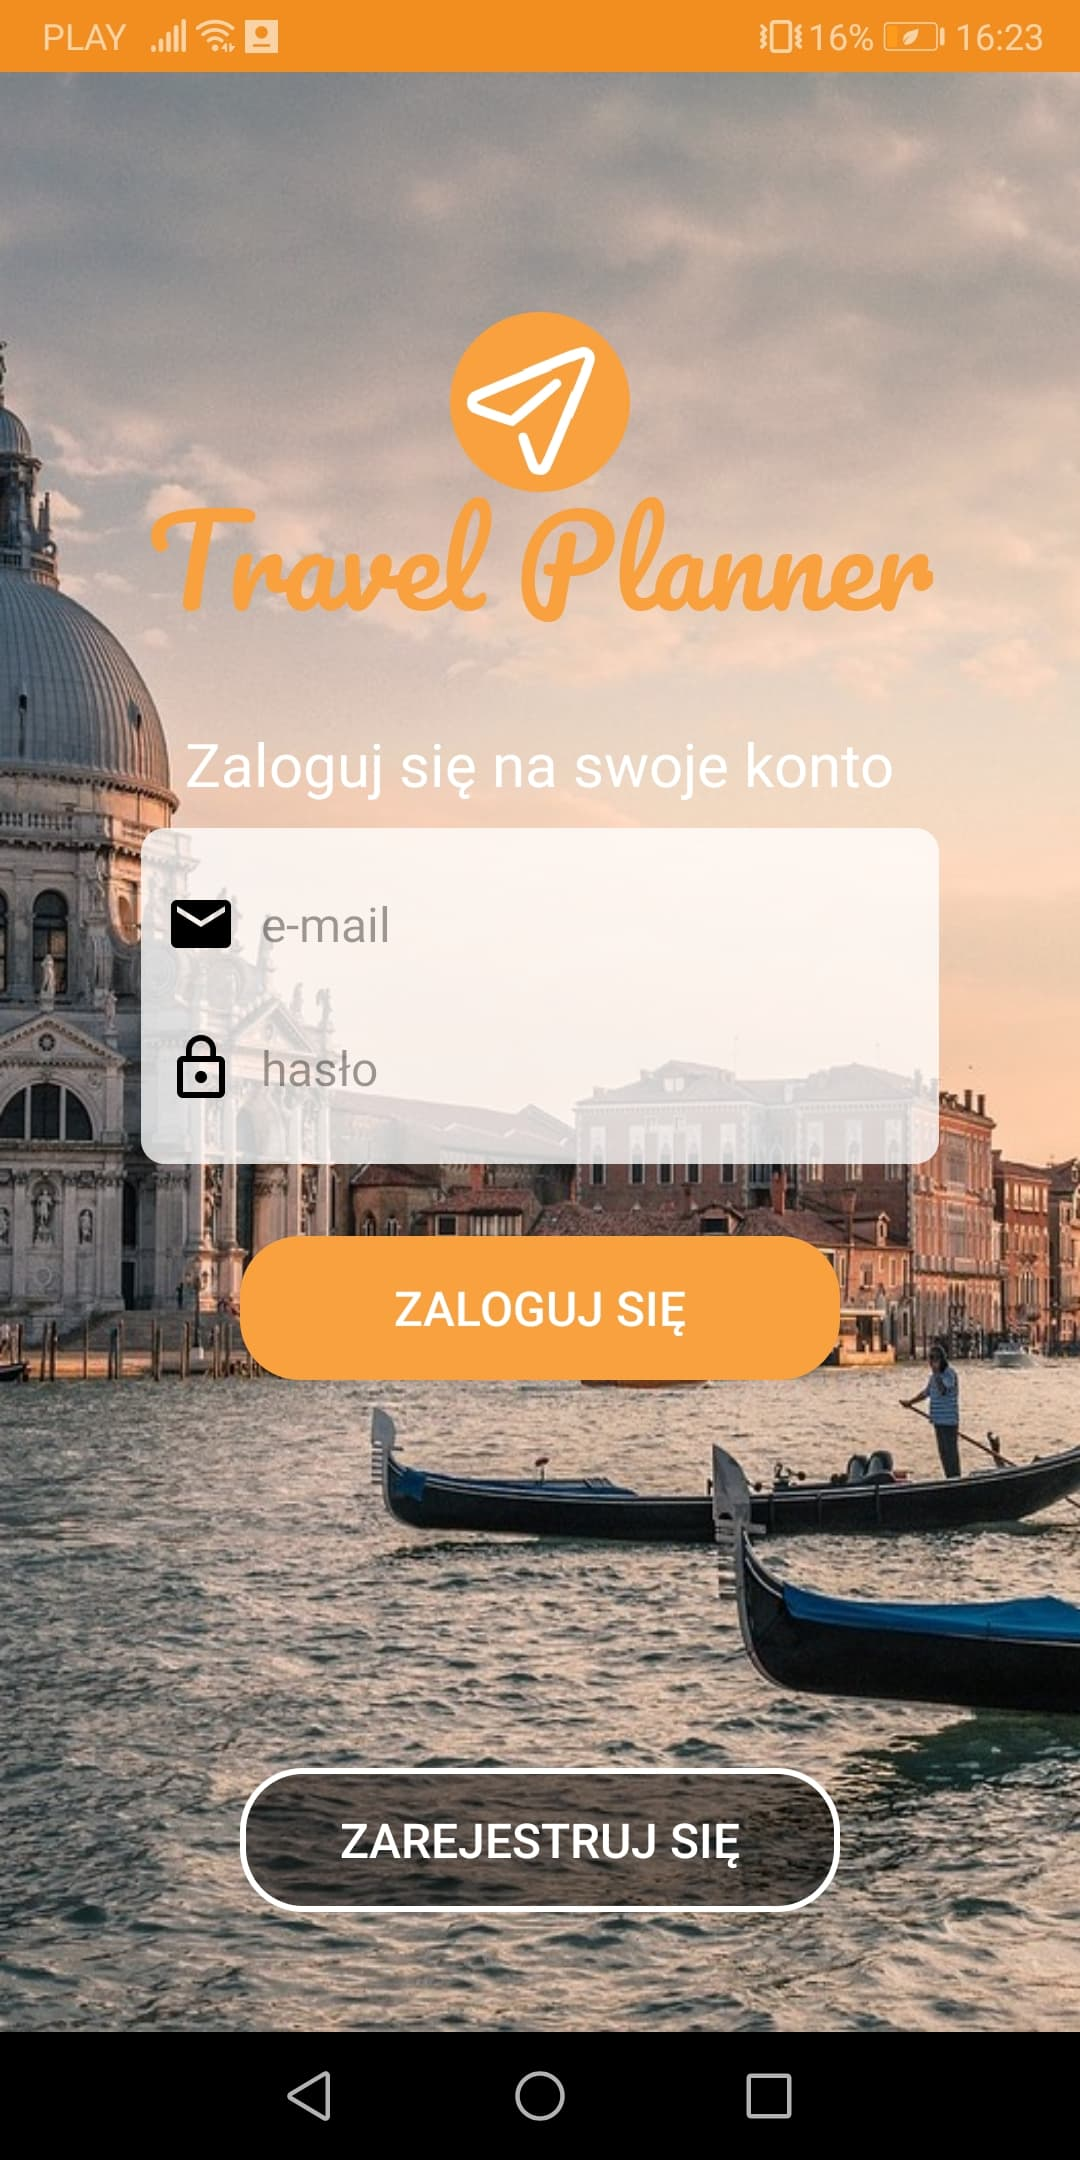
\includegraphics[width=0.4\textwidth]{loginView}}
\hfill
\subfloat[Widok rejestracji.\label{fig:registrationPage}]{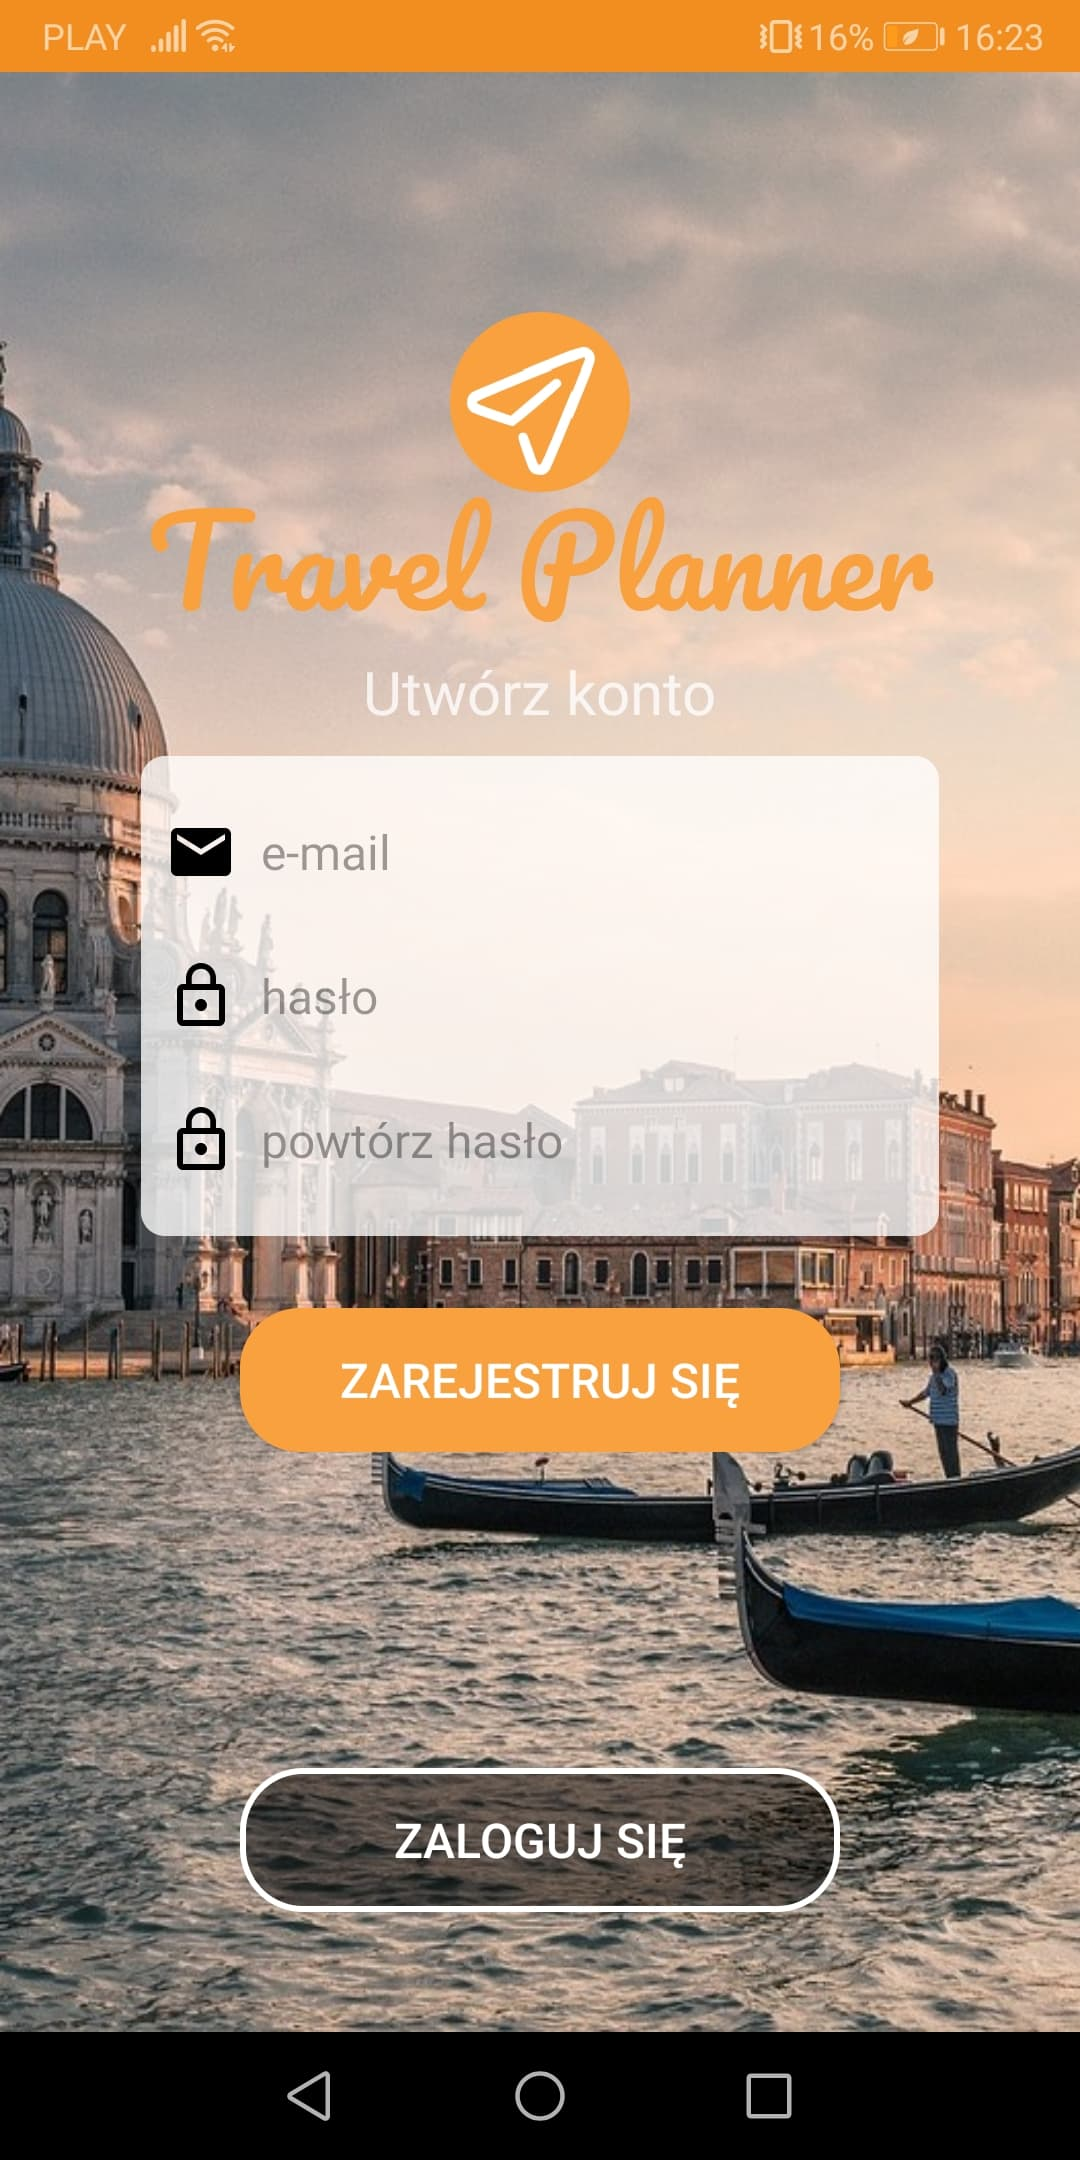
\includegraphics[width=0.4\textwidth]{registrationPage}}
\hfill\null

\caption{Logowanie i rejestracja użytkownika.}
\label{fig:podrecznik1}
\end{figure}
\FloatBarrier

\section{Podróże}
Pierwszy widok pojawiający się tuż po zalogowaniu zawiera listę dostępnych podróży (rys. 10.3a).

\subsection{Tworzenie podróży}
W celu utworzenia podróży należy:
\begin{enumerate}
\item Nacisnąć przycisk oznaczony symbolem \textit{+}.
\item Uzupełnić okno dialogowe nazwą podróży i kliknąć \textit{OK} (rys. 10.3b).
\item Utworzona podróż pojawi się na liście wraz z domyślnym zdjęciem (rys. 10.3c).
\end{enumerate}

\section{Widok podróży}
Po wybraniu danej podróży zostaje wyświetlony widok zawierający informacje na jej temat.

\subsection{Zmiana nazwy podróży}

W celu zmiany nazwy podróży należy:
\begin{enumerate}
\item Nacisnąć przycisk oznaczony symbolem ołówka.
\item Uzupełnić okno dialogowe nową nazwą podróży i kliknąć \textit{OK}.
\item Nazwa podróży zostanie zaktualizowana.
\end{enumerate}

\begin{figure}[h]
\centering
\null\hfill
\subfloat[Widok podróży użytkownika.\label{fig:travelsView}]{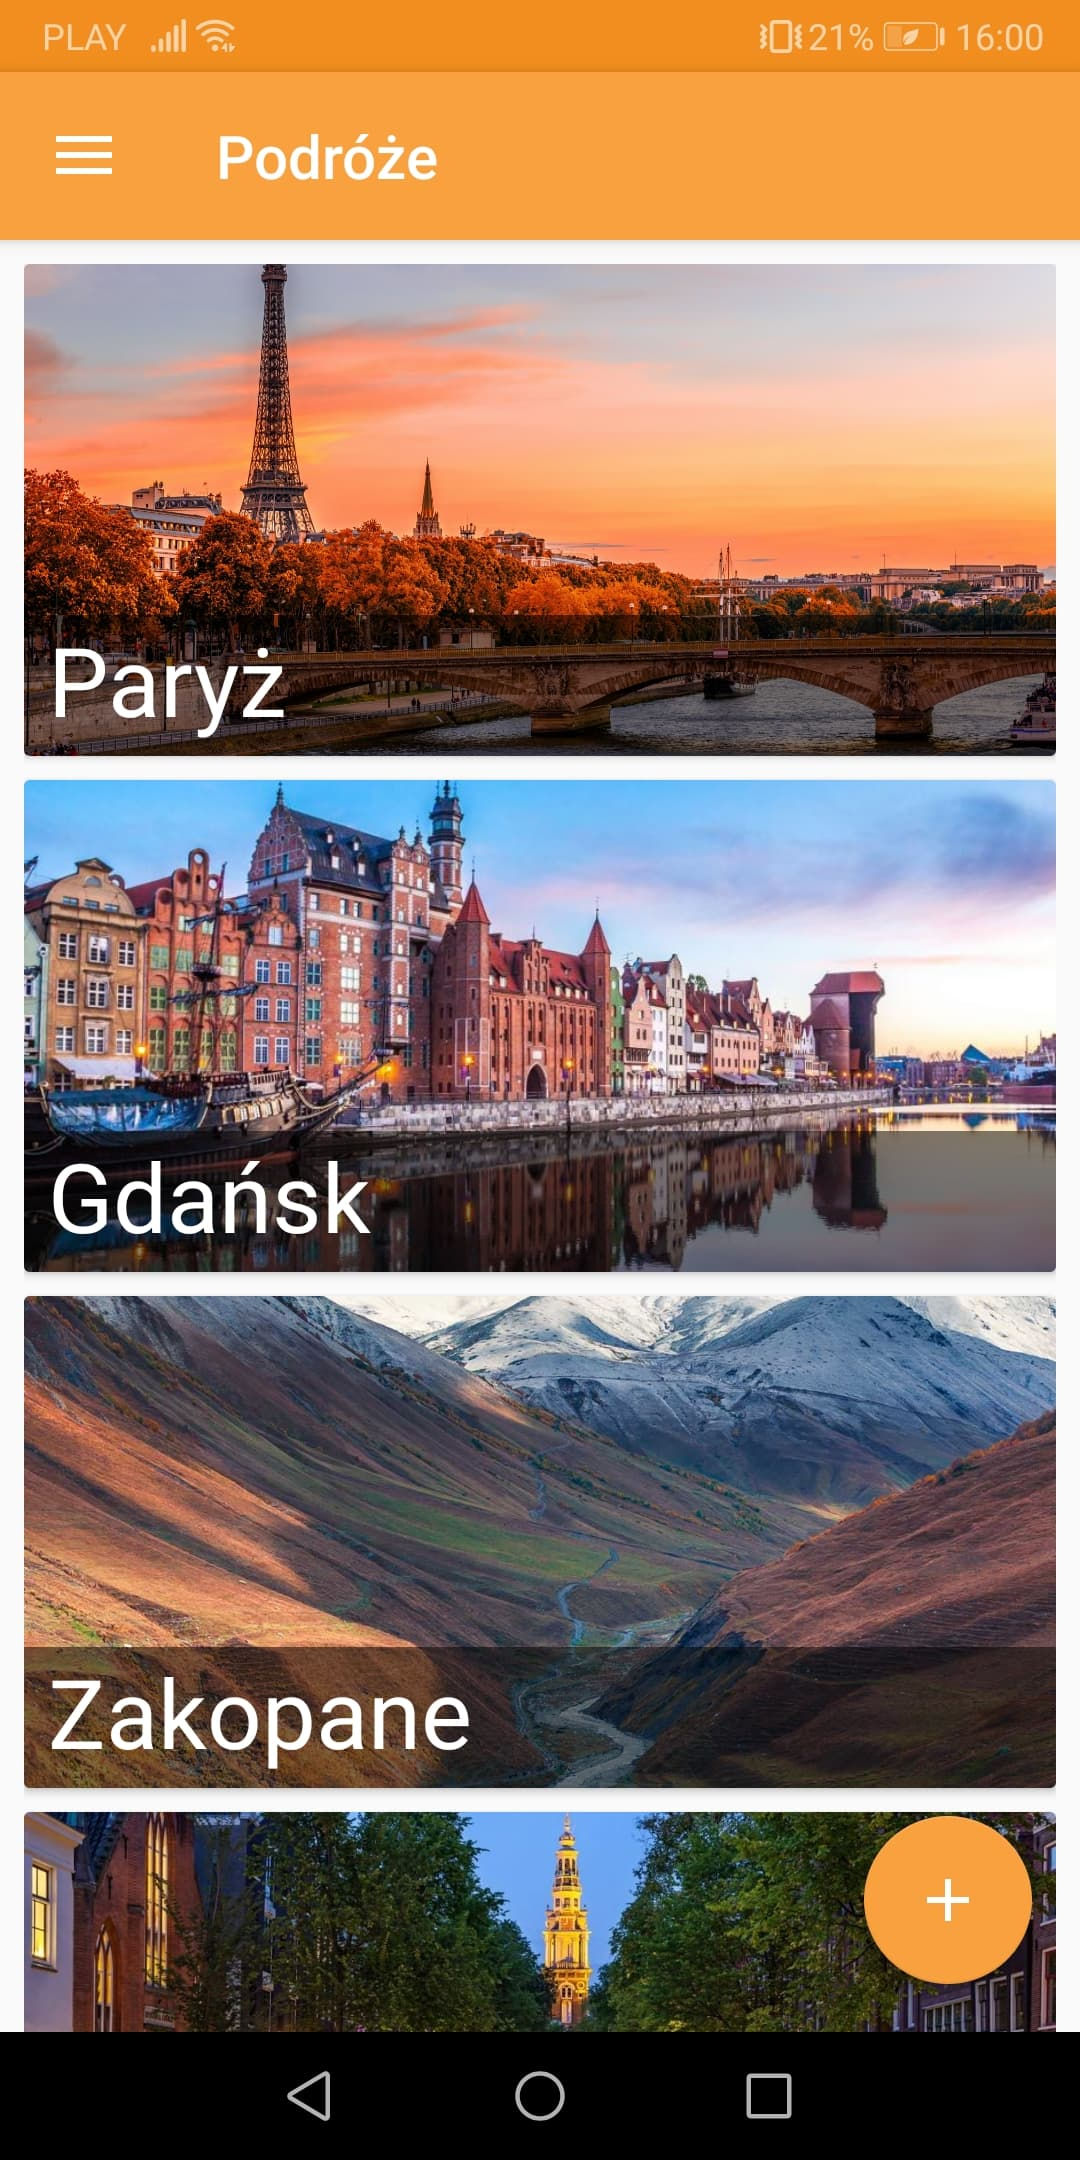
\includegraphics[width=0.32\textwidth]{travelsView}}
\hfill
\subfloat[Okno dialogowe.\label{fig:createNewTravel}]{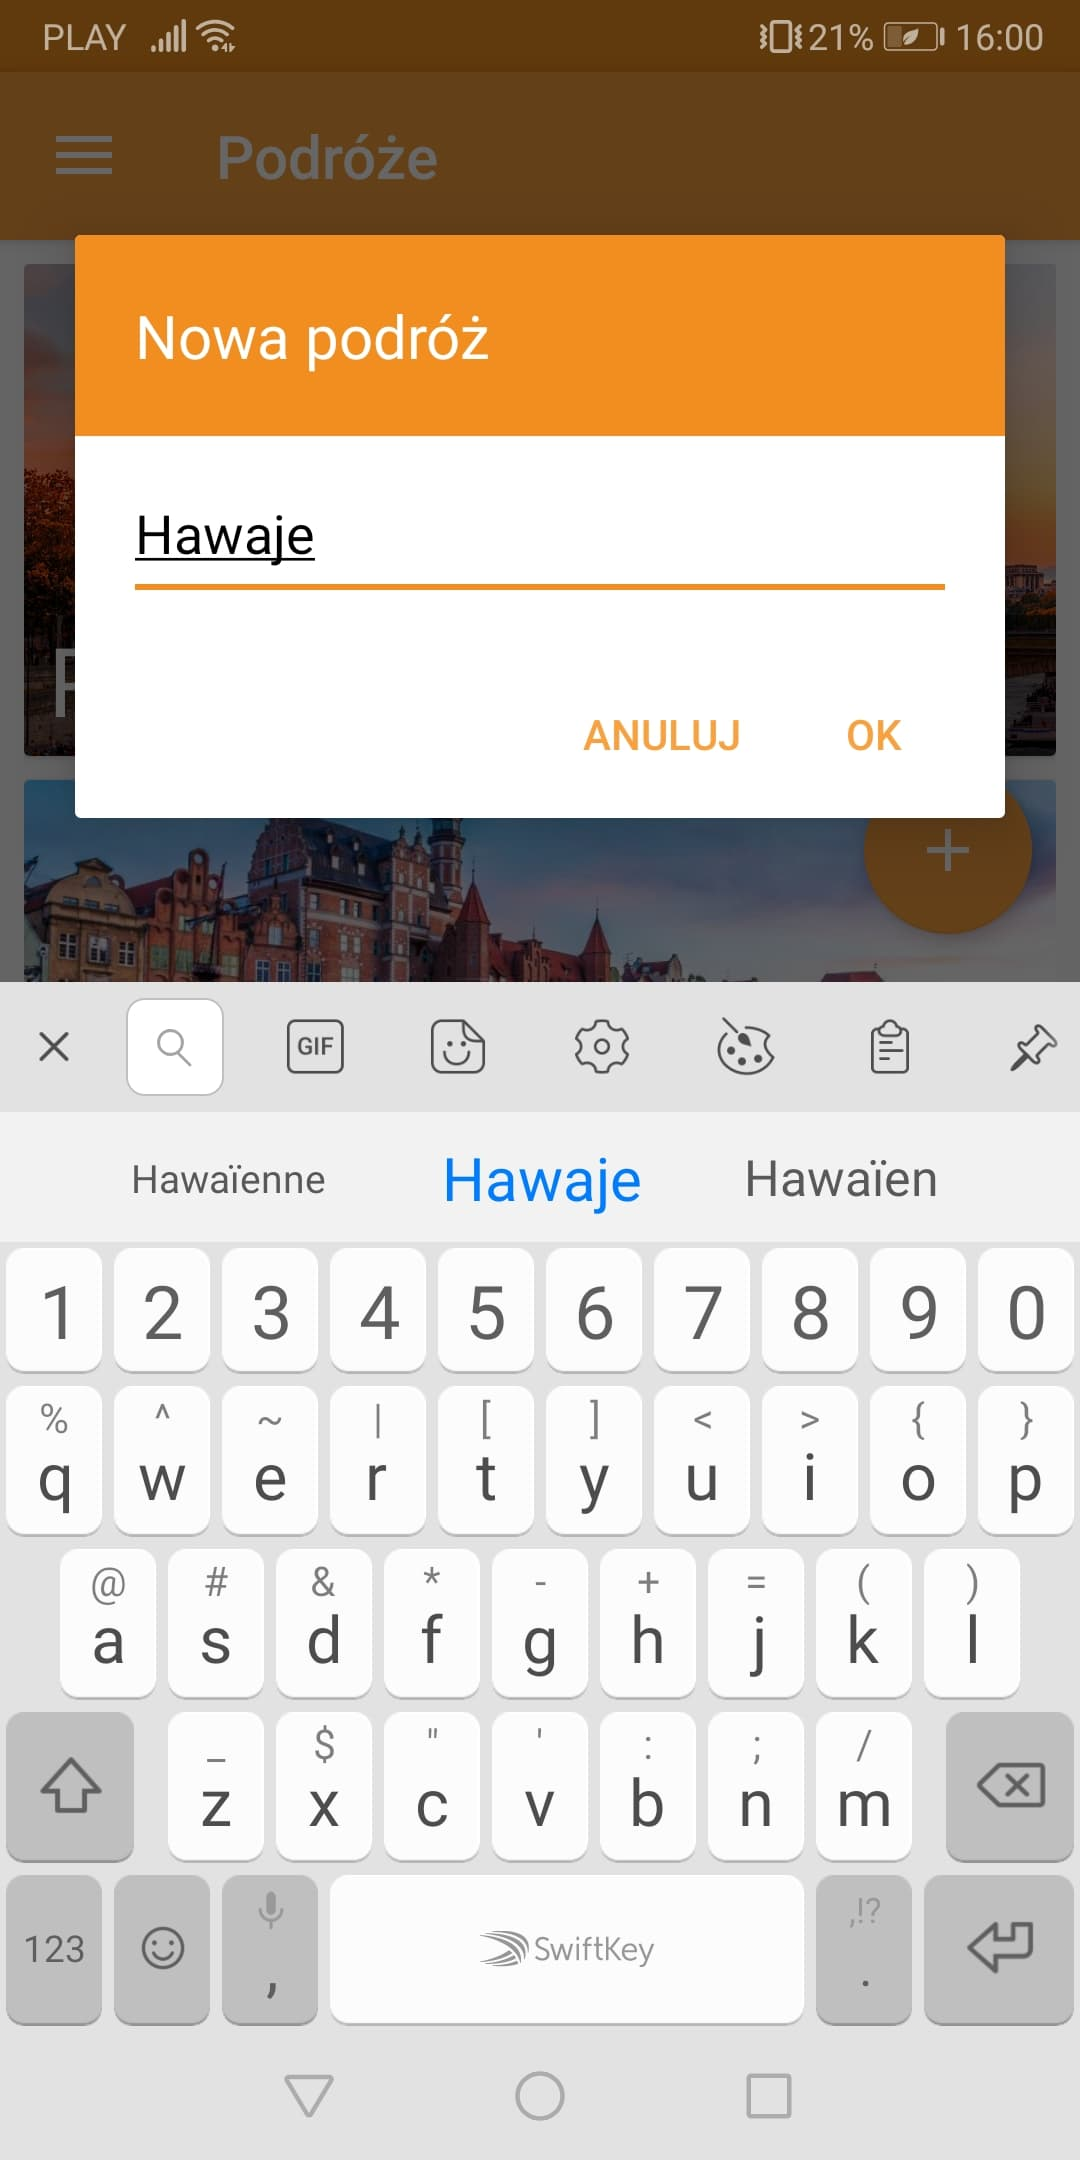
\includegraphics[width=0.32\textwidth]{createNewTravel}}
\hfill
\subfloat[Domyślny obraz podróży.\label{fig:defaultImage}]{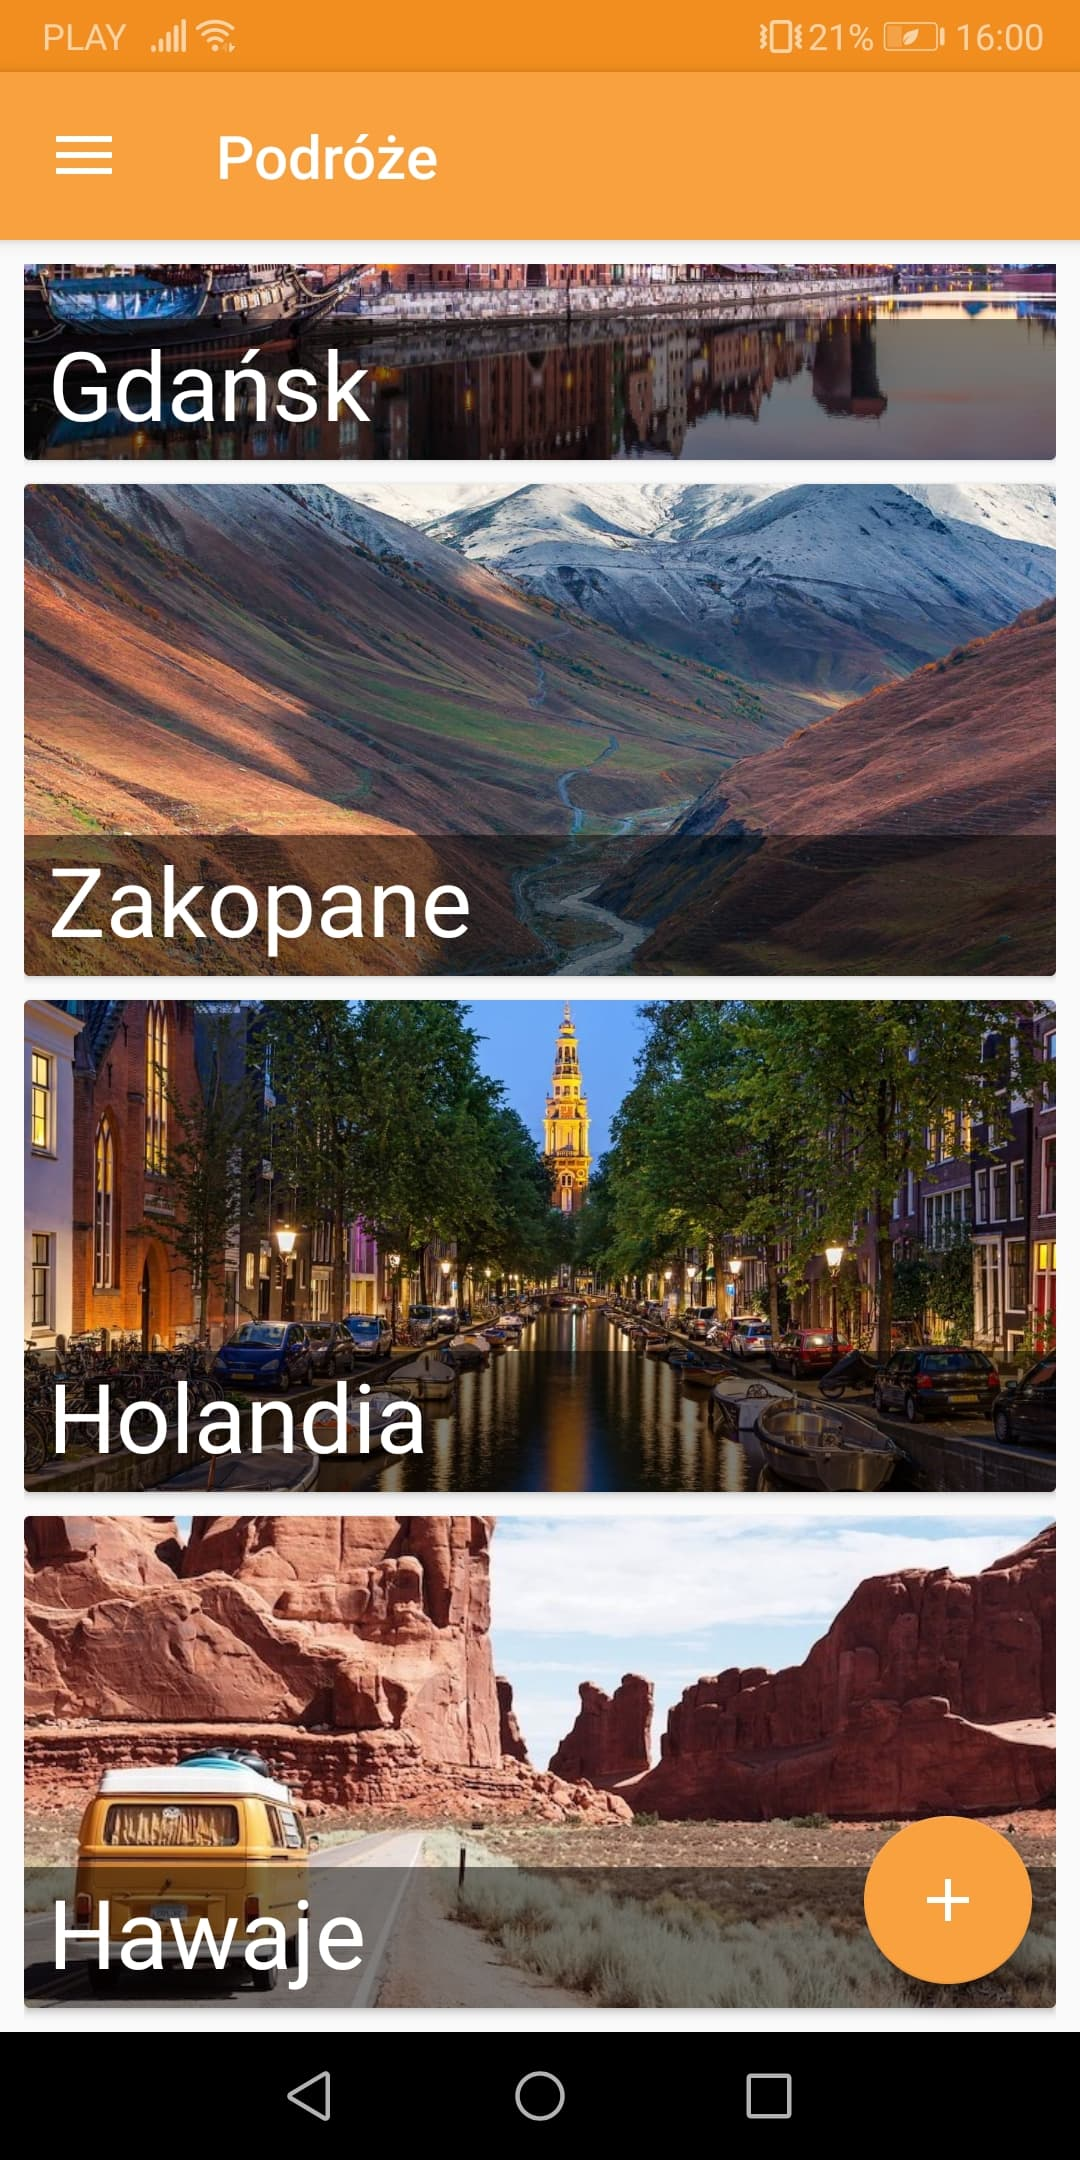
\includegraphics[width=0.32\textwidth]{defaultImage}}
\hfill\null

\caption{Tworzenie nowej podróży}
\label{fig:podrecznik2}
\end{figure}
\FloatBarrier

\begin{figure}[h]
\centering

\centering
\null\hfill
\subfloat[Widok danej podróży.\label{fig:newTravel}]{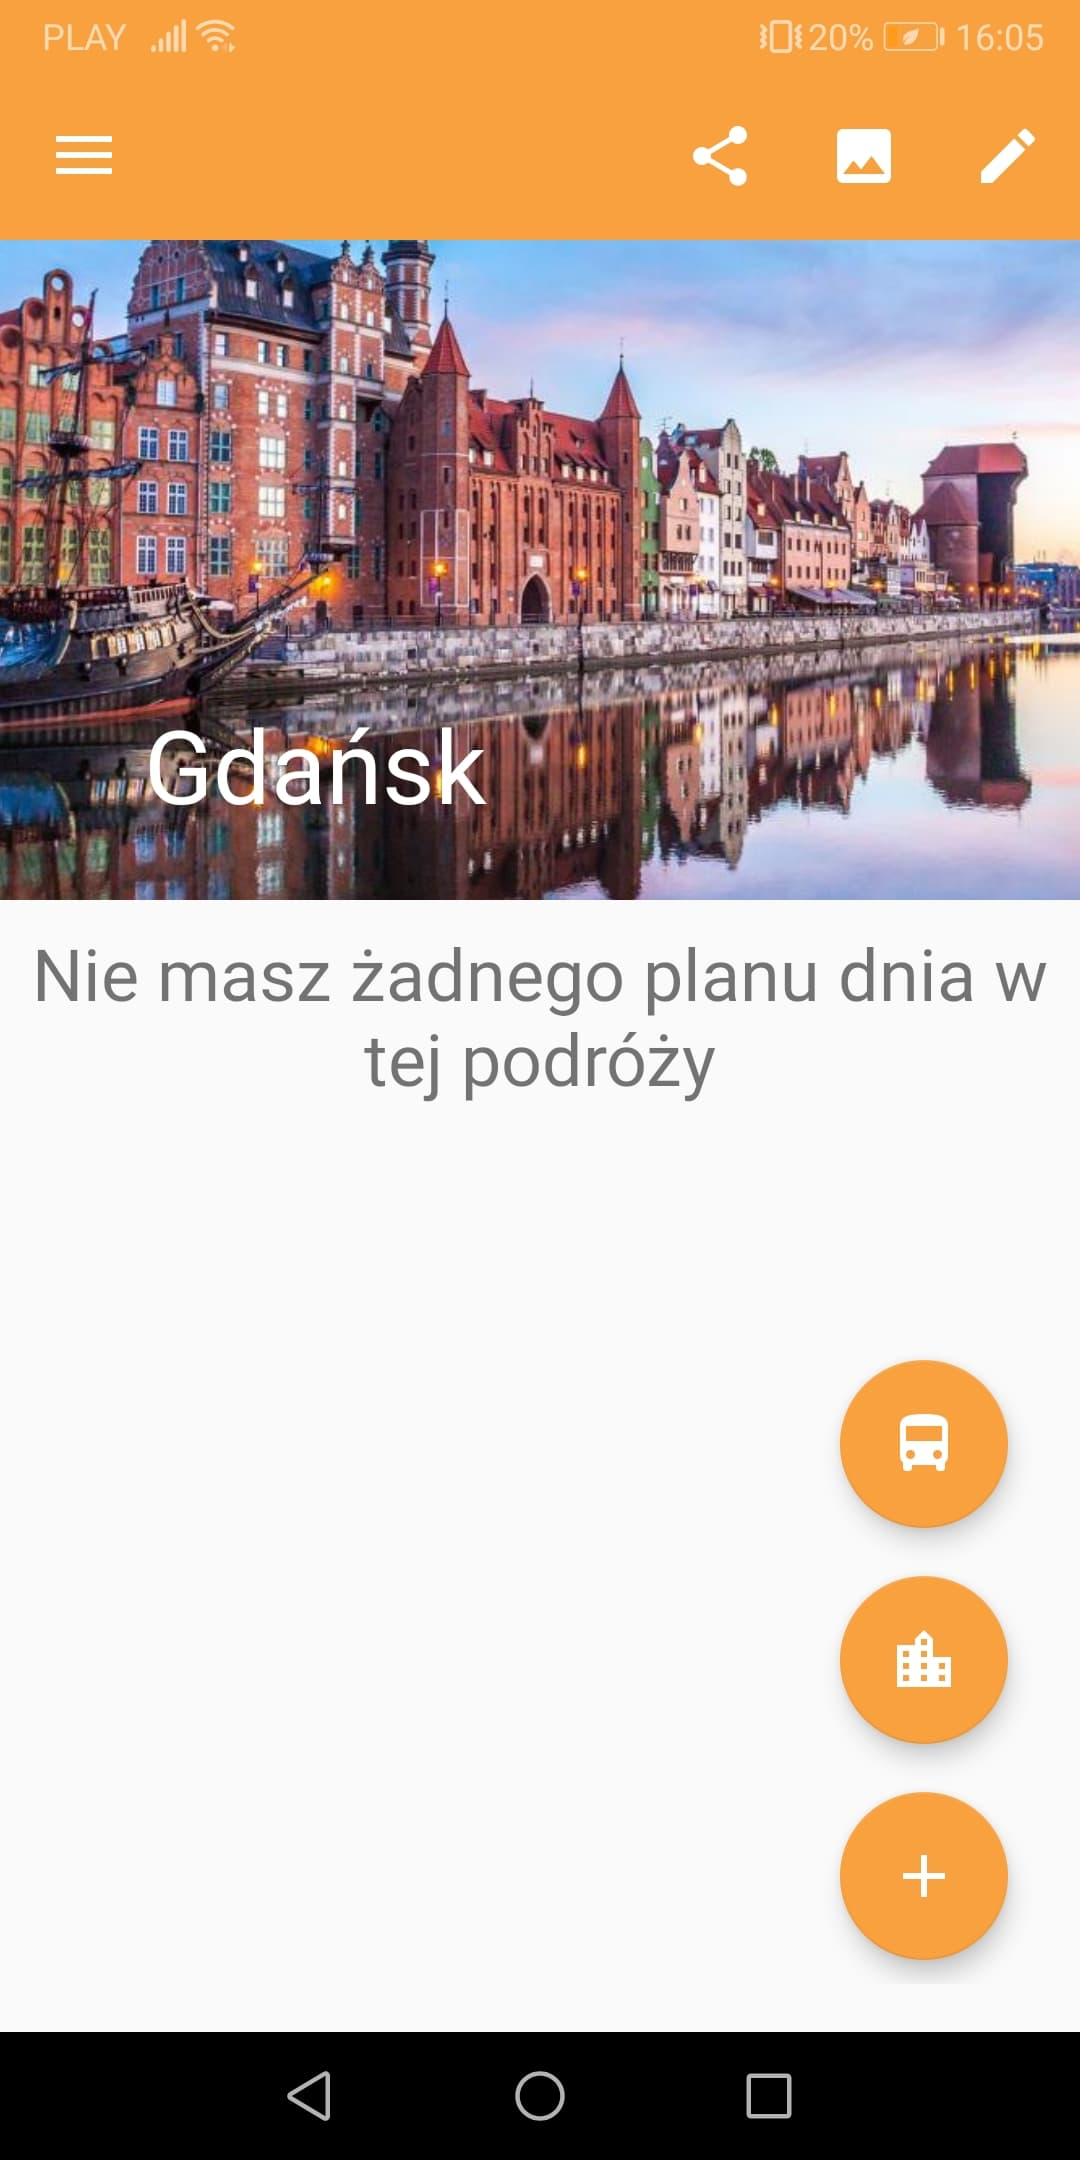
\includegraphics[width=0.4\textwidth]{newTravel}}
\hfill
\subfloat[Udostępnianie podróży znajomym.\label{fig:shareTravelDialog}]{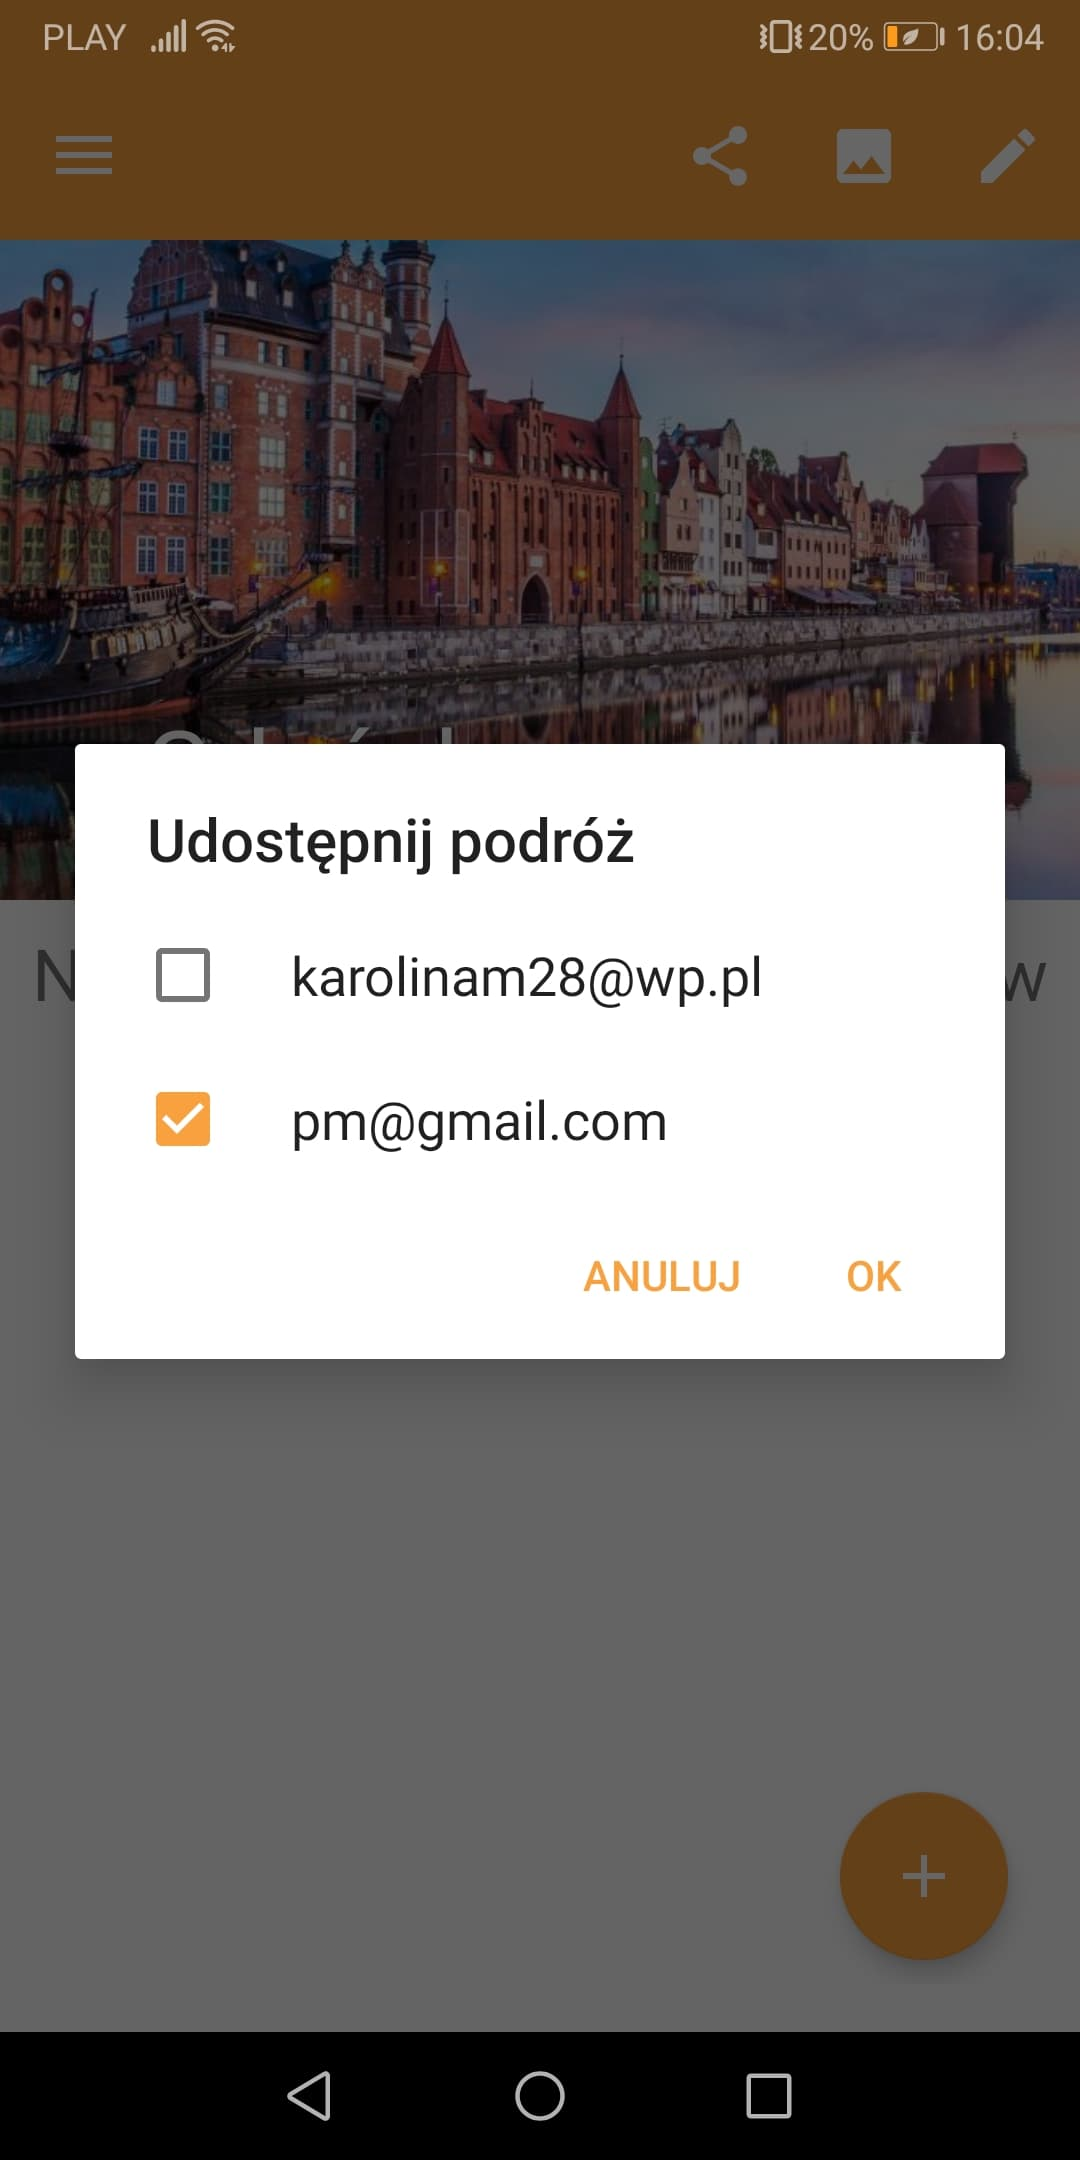
\includegraphics[width=0.4\textwidth]{shareTravelDialog}}
\hfill\null

\caption{Pojedyncza podróż.}
\label{fig:podrecznik3}
\end{figure}
\FloatBarrier

\subsection{Zmiana tła podróży}

W celu zmiany tła podróży należy:
\begin{enumerate}
\item Nacisnąć przycisk oznaczony symbolem zdjęcia (rys. 10.4a).
\item Wybrać odpowiednie zdjęcie z galerii urządzenia.
\item Zdjęcie zostanie zaktualizowane.
\end{enumerate}

\subsection{Udostępnianie podróży znajomym}

W celu udostępnienia podróży znajomym należy:
\begin{enumerate}
\item Nacisnąć przycisk oznaczony symbolem udostępniania.
\item Wybrać wszystkich znajomych, którym ma zostać udostępniona podróż (rys. 10.4b).
\item Potwierdzić swój wybór poprzez naciśnięcie przycisku \textit{OK}.
\item W przypadku potwierdzenia wykonania czynności pojawi się powiadomienie z odpowiednim komunikatem.
\end{enumerate}

\subsection{Dodanie elementu planu dnia}
W celu dodania elementu planu dnia należy:
\begin{enumerate}
\item Nacisnąć przycisk oznaczony symbolem \textit{+}.
\item Wybrać jedną z dwóch dostępnych opcji.
\end{enumerate}

\par Pierwsza z opcji jest oznaczona poprzez symbol budynku.
Umożliwia on dodanie miejsca do planu dnia.

\begin{enumerate}
\item Należy wybrać kategorię spośród między innymi (rys. 10.5a):
\begin{itemize}
\item jedzenie i picie,
\item restauracja,
\item rozrywka,
\item zabytki i muzea,
\item nocleg,
\item zakupy,
\item aktywny wypoczynek,
\item natura,
\item stacja paliw.
\end{itemize}
\item Po naciśnięciu wyszukiwania miejsca po nazwie pojawia się widok mapy umożliwiającej wybranie konkretnego miejsca (rys. 10.5b).
\item Po wybraniu pinezki pojawiają się dokładne informacje na temat miejsca (rys. 10.5c).
\item Naciśnięcie przycisku zawierającego symbol odhaczenia (ang.tick) przekierowuje użytkownika do pierwszego ekranu wyszukiwania.
\item Następnie należy wybrać datę oraz godzinę realizacji planu (rys. 10.5d oraz rys.10.5e).
\item Opcjonalne jest dodanie własnych notatek.
\item Dodanie miejsca następuje po naciśnięciu przycisku oznaczonym symbolem odhaczenia (ang.tick).
\end{enumerate}

\begin{figure}[h]

\centering
\null\hfill
\subfloat[Uzupełnienie danych.\label{fig:searchPlace}]{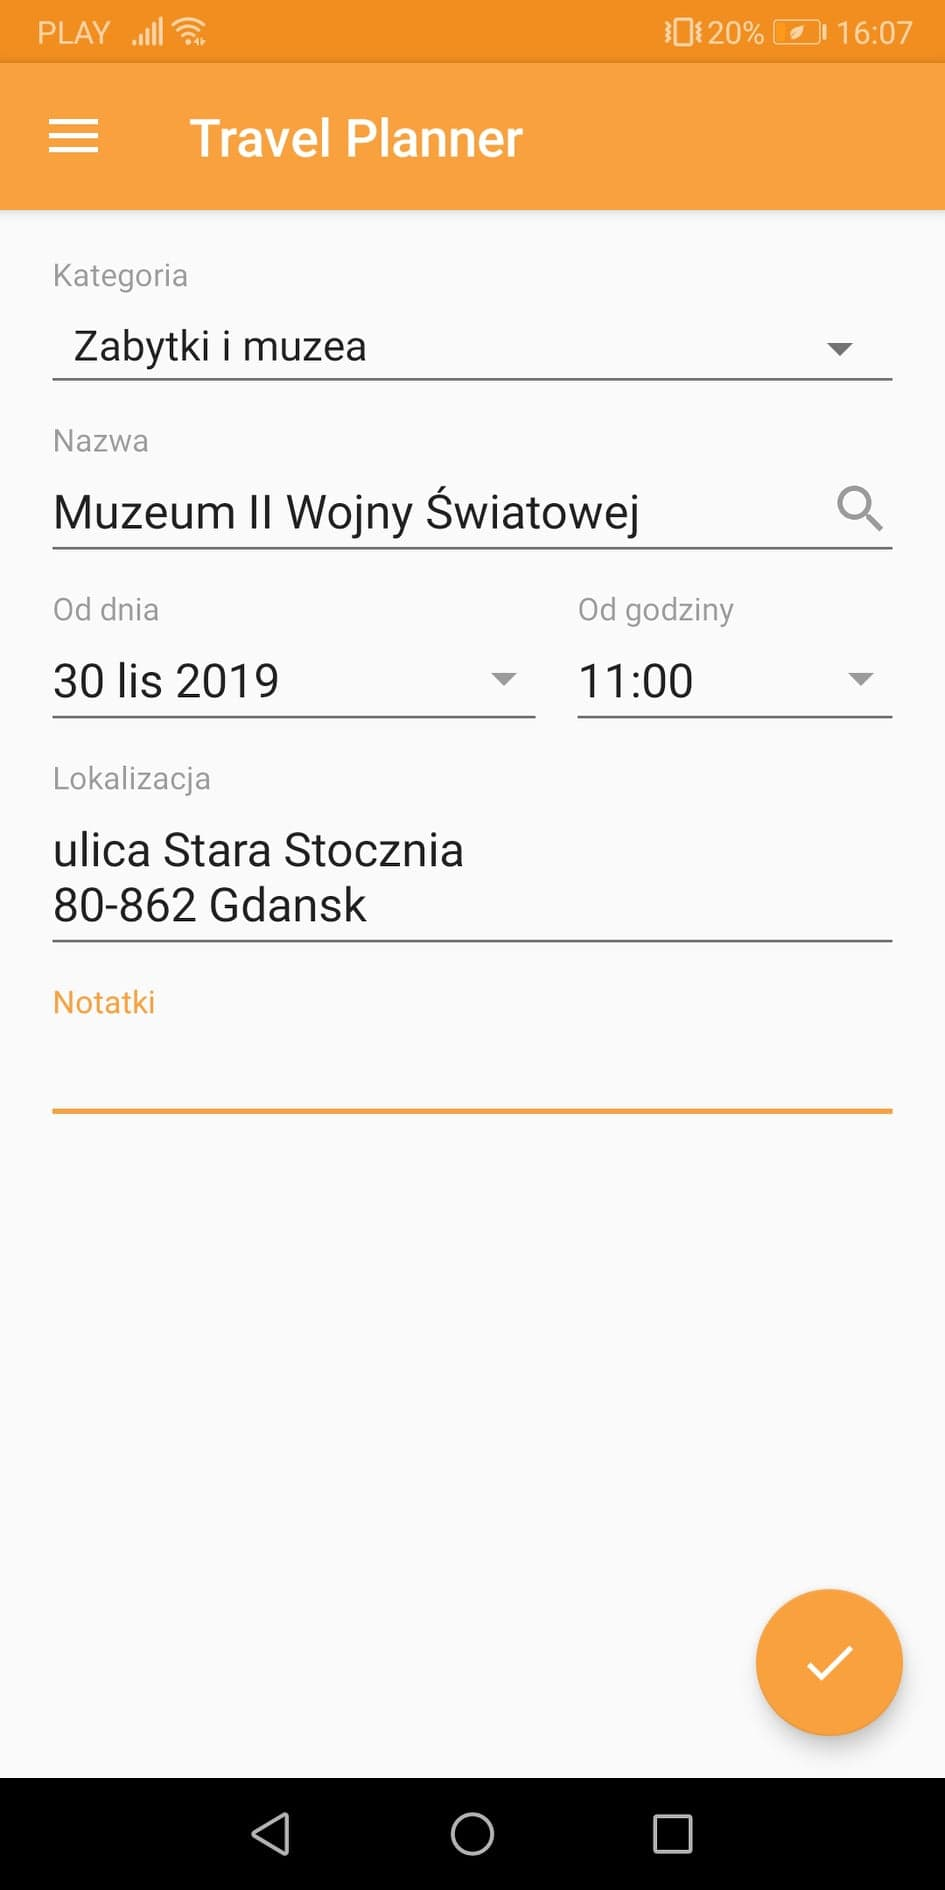
\includegraphics[width=0.32\textwidth]{searchPlace}}
\hfill
\subfloat[Wyszukiwanie miejsca.\label{fig:searchingPlace}]{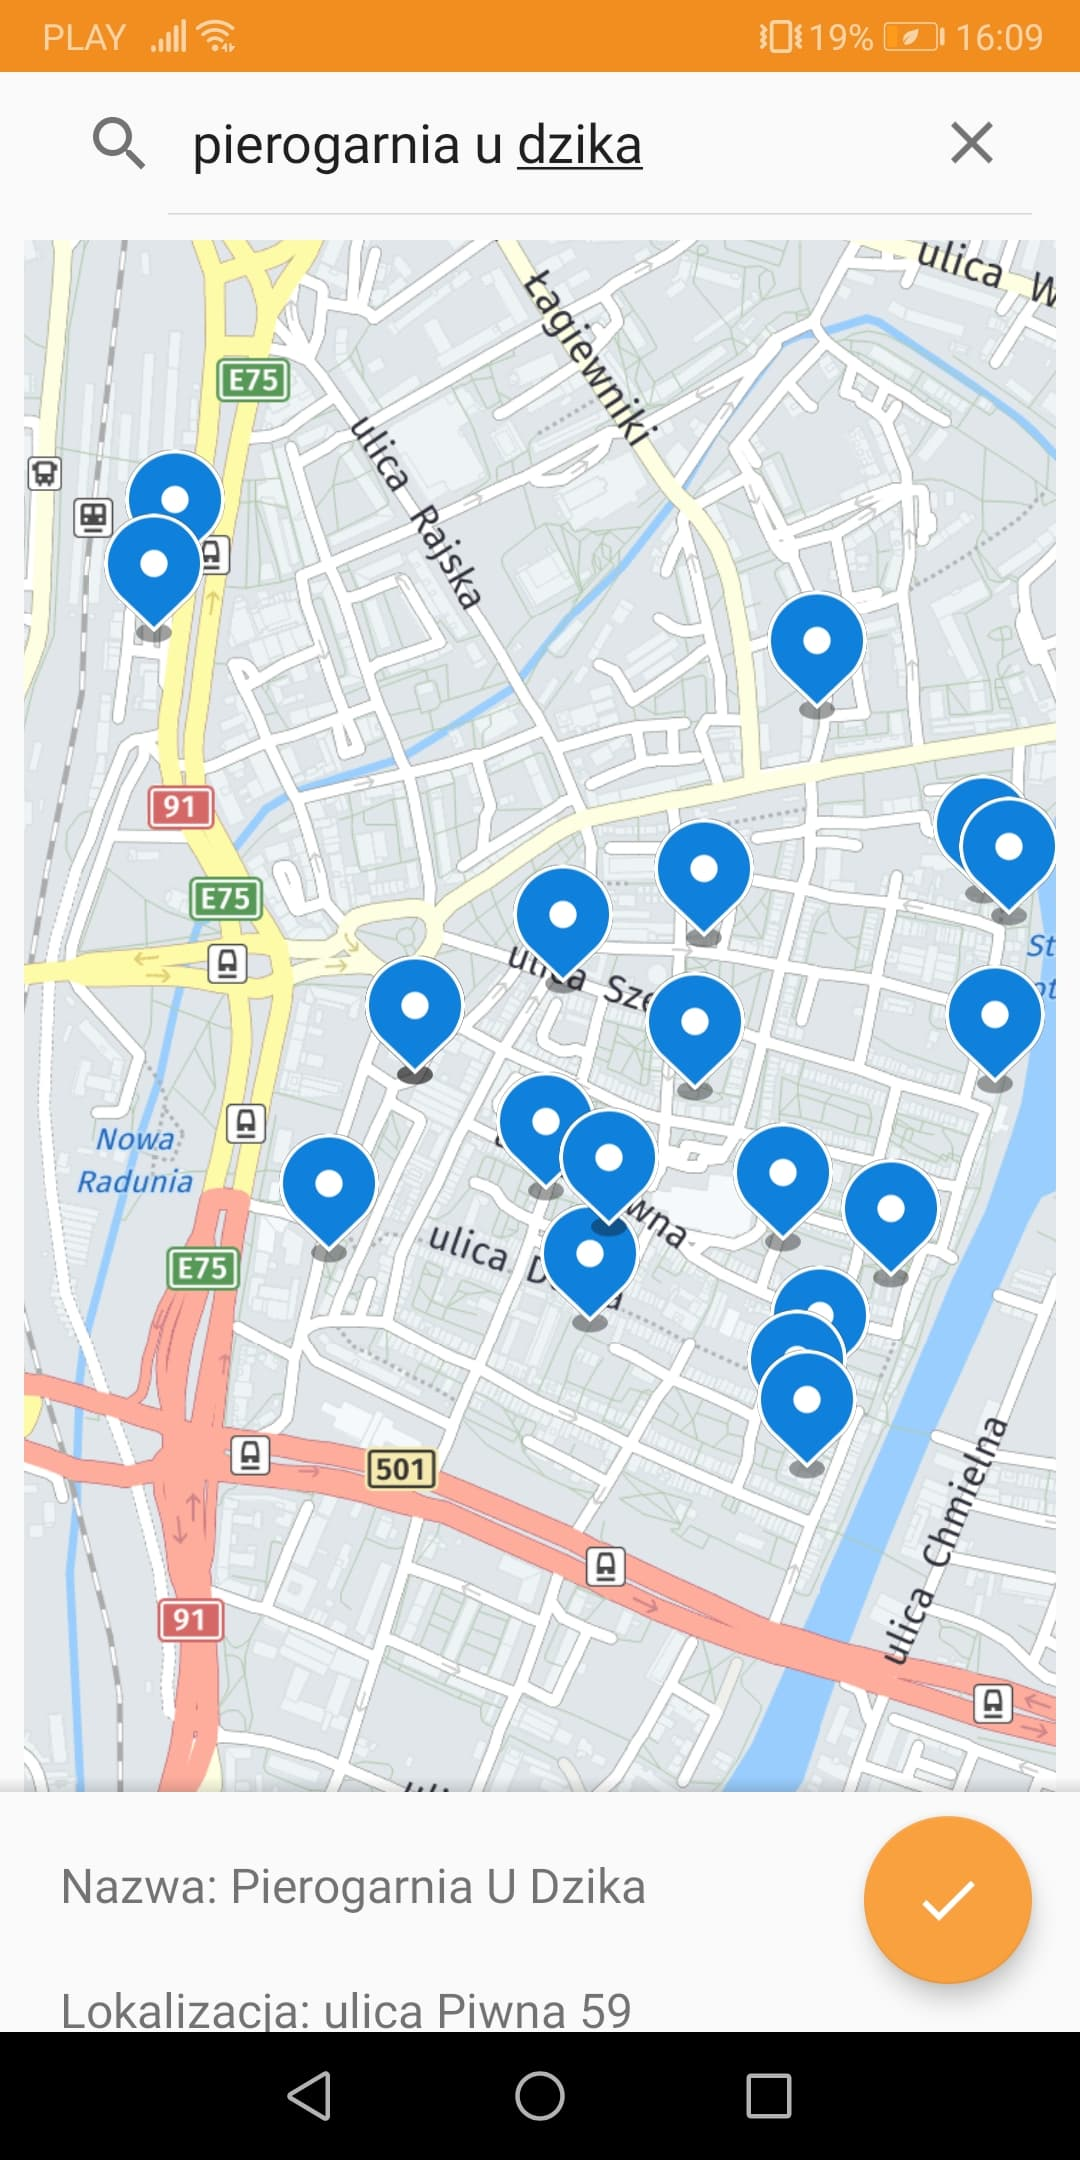
\includegraphics[width=0.32\textwidth]{searchingPlace}}
\hfill
\subfloat[Szczegółowe informacje na temat miejsca.\label{fig:placeDescription}]{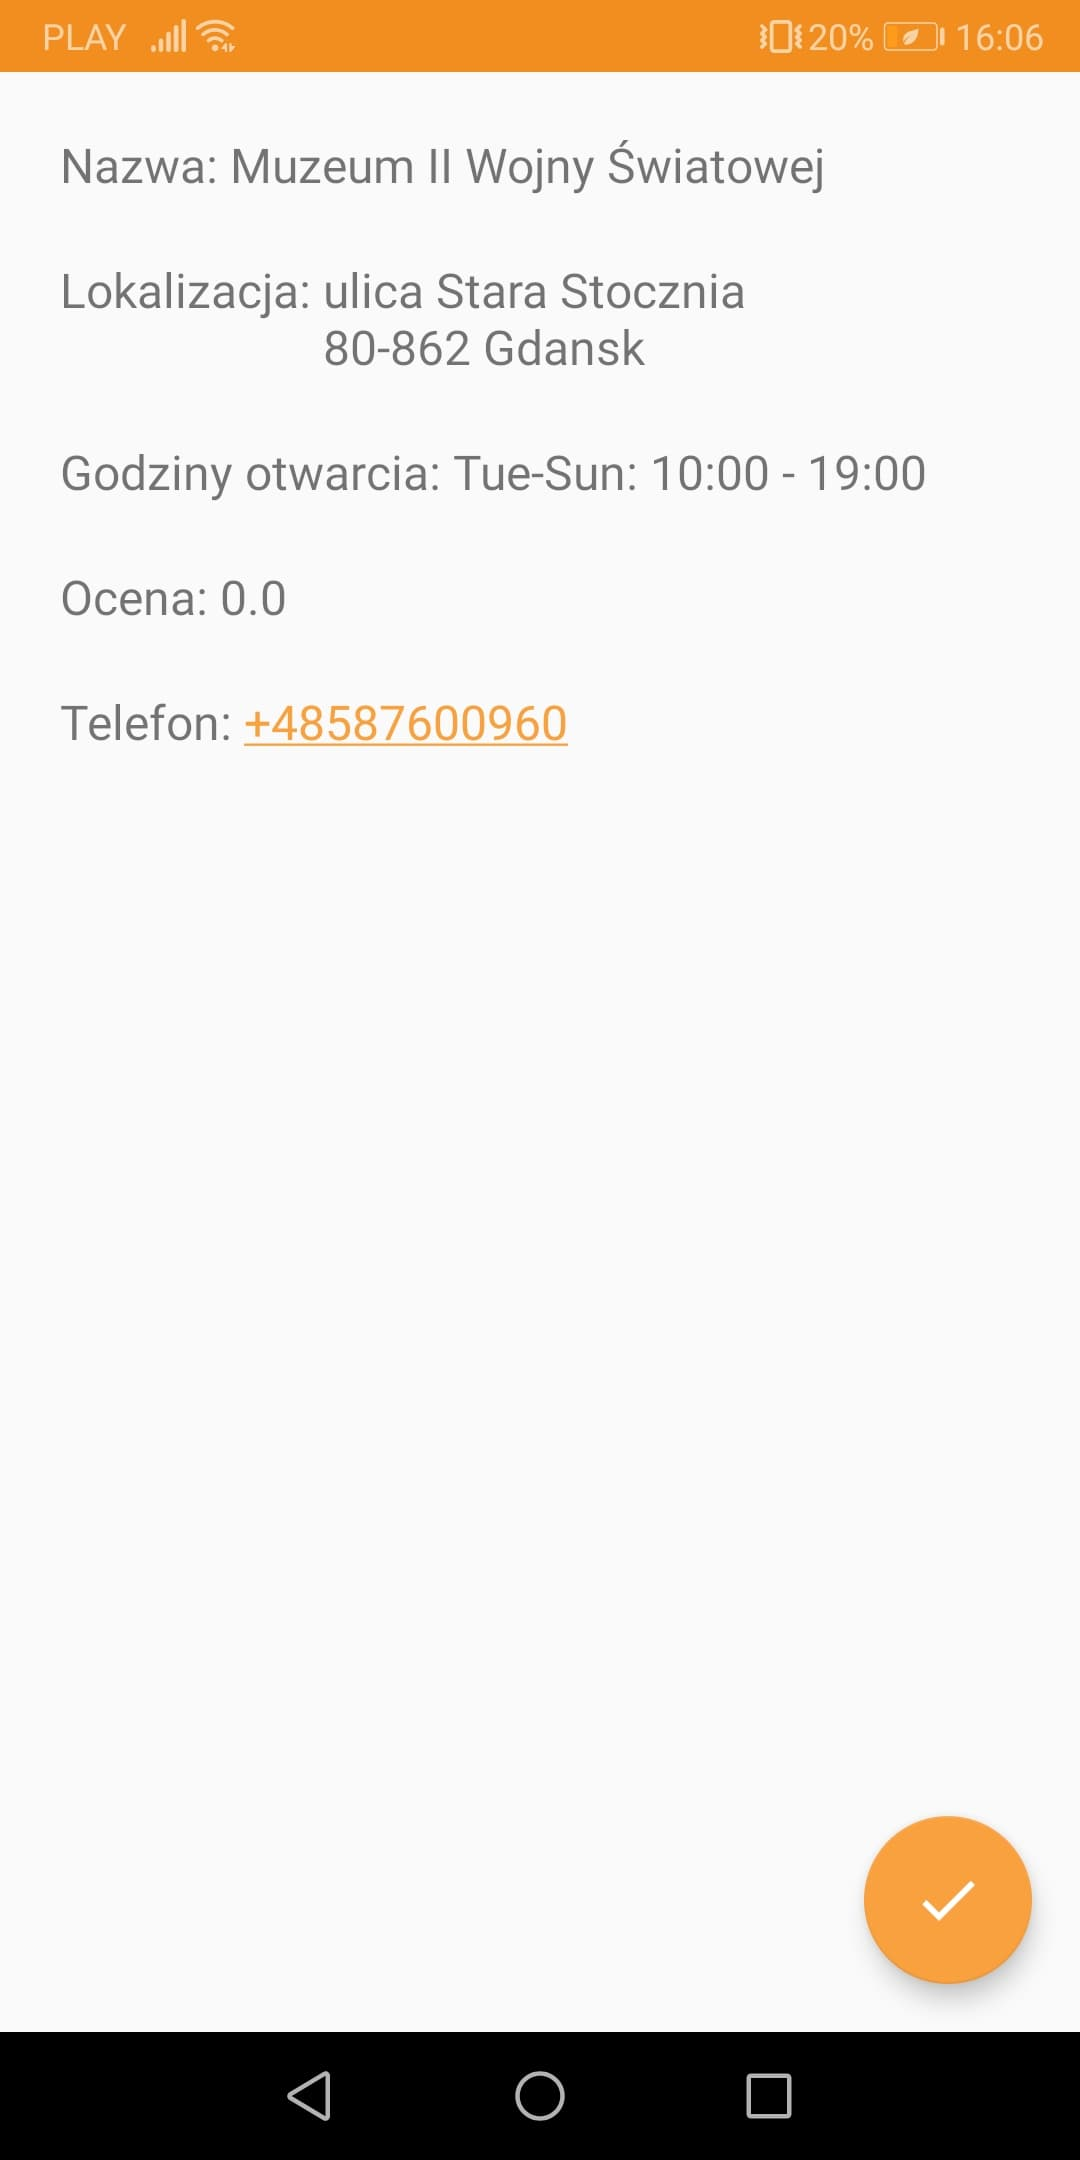
\includegraphics[width=0.32\textwidth]{placeDescription}}
\hfill\null

\null\hfill
\centering
\subfloat[Wybieranie daty.\label{fig:clock}]{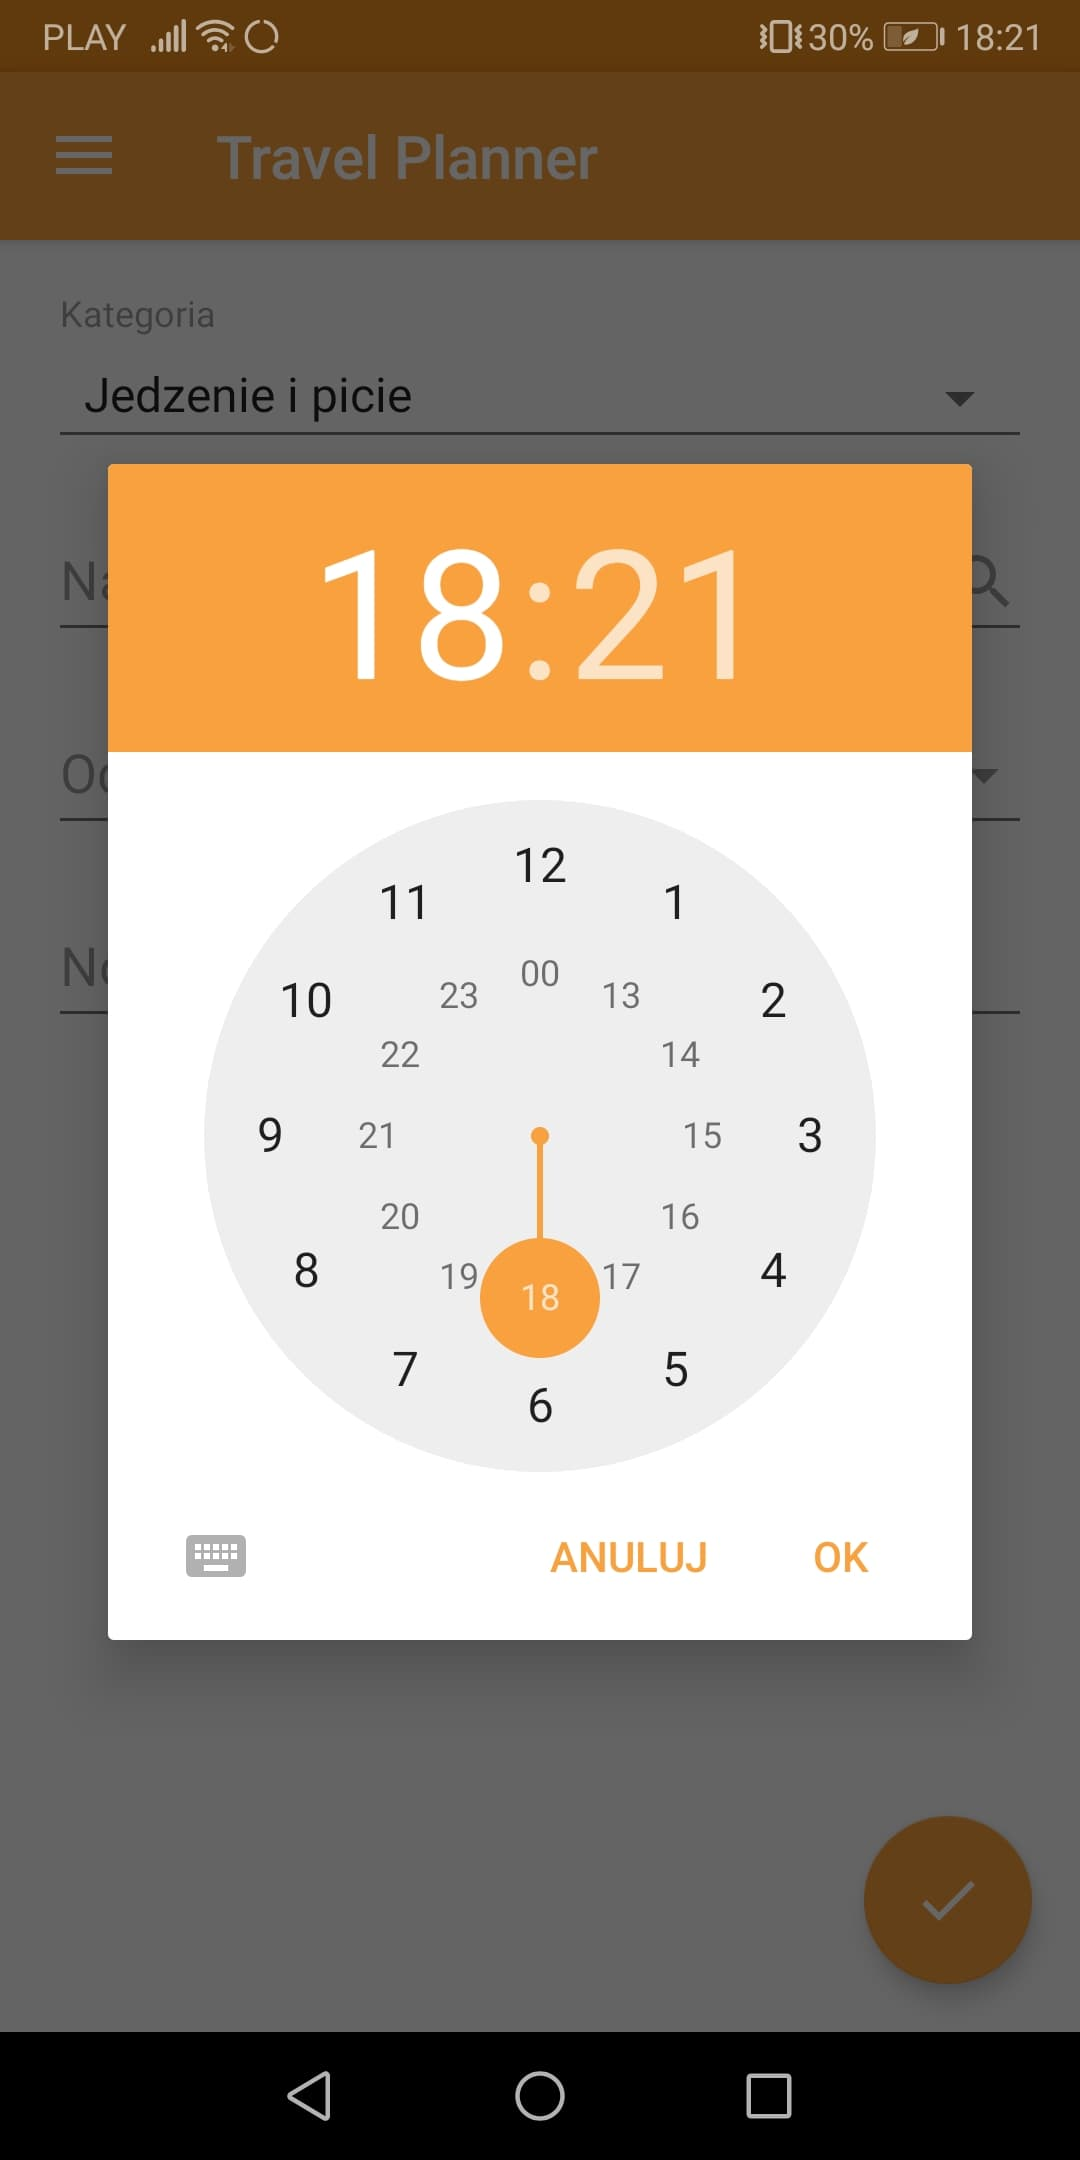
\includegraphics[width=0.32\textwidth]{clock}}
\hfill
\subfloat[Udostępnianie podróży znajomym.\label{fig:calendar}]{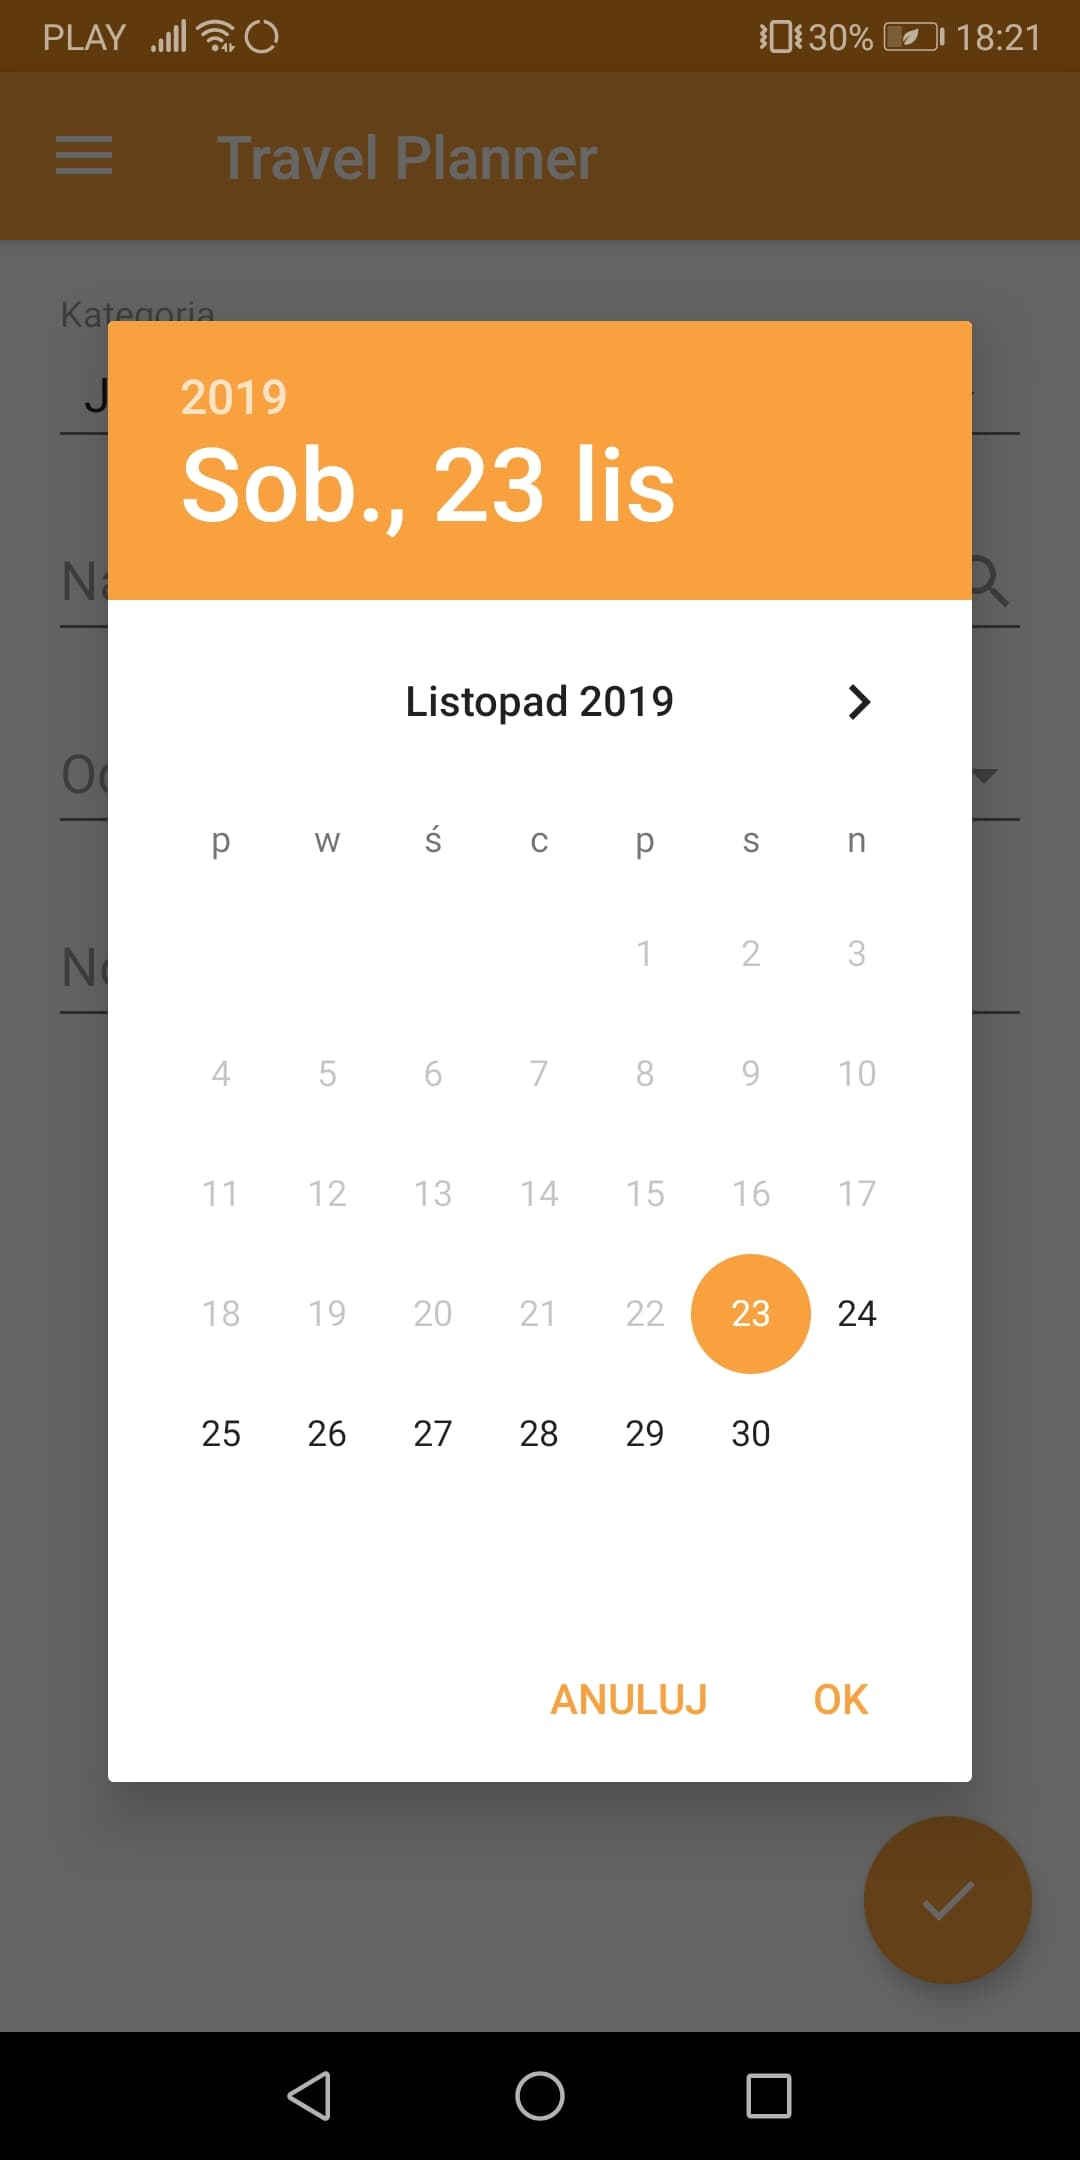
\includegraphics[width=0.32\textwidth]{calendar}}
\hfill\null
\caption{Tworzenie elementu planu dnia.}
\label{fig:podrecznik7}
\end{figure}
\FloatBarrier

W przypadku wybrania przycisku z symbolem samochodu użytkownik ma możliwość dodania transportu jako element planu dnia.
\begin{enumerate}
\item Należy kliknąć na na pole miejsca początkowego (rys. 10.6a).
\item Następnie wybrać element planu dnia.
\item Kliknąć na pole miejsca docelowego.
\item Wybrać element planu dnia.
\item Kliknąć na przycisk oznaczony symbolem strzałki w prawo.
\item Wybrać rodzaj transportu (rys. 10.6b).
\item Kliknąć na przycisk oznaczony symbolem lupy.
\end{enumerate}

\begin{figure}[h]

\centering
\null\hfill
\subfloat[Formularz wyszukiwania.\label{fig:transport1}]{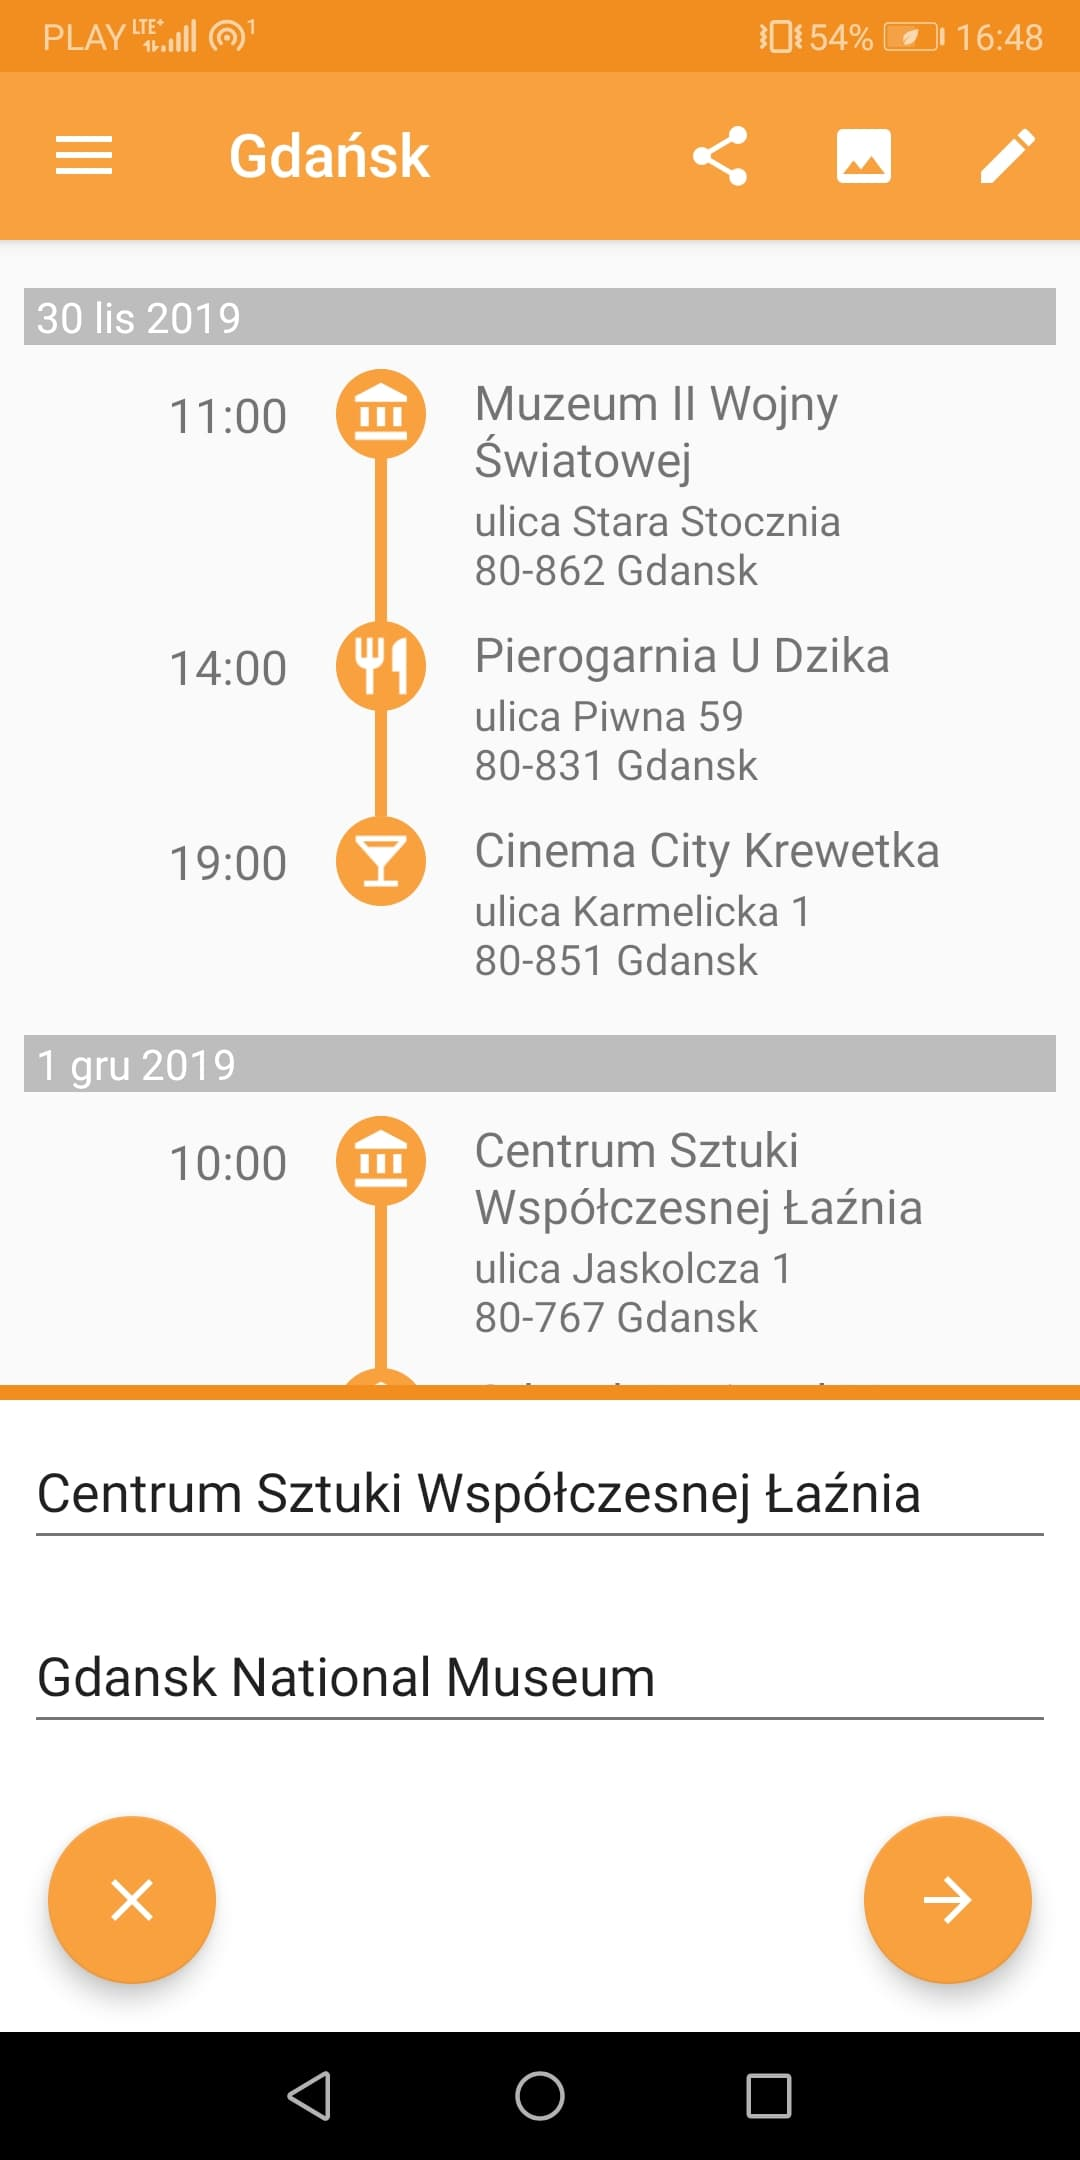
\includegraphics[width=0.4\textwidth]{transport1}}
\hfill
\subfloat[Wynik wyszukiwania\label{fig:transport2}]{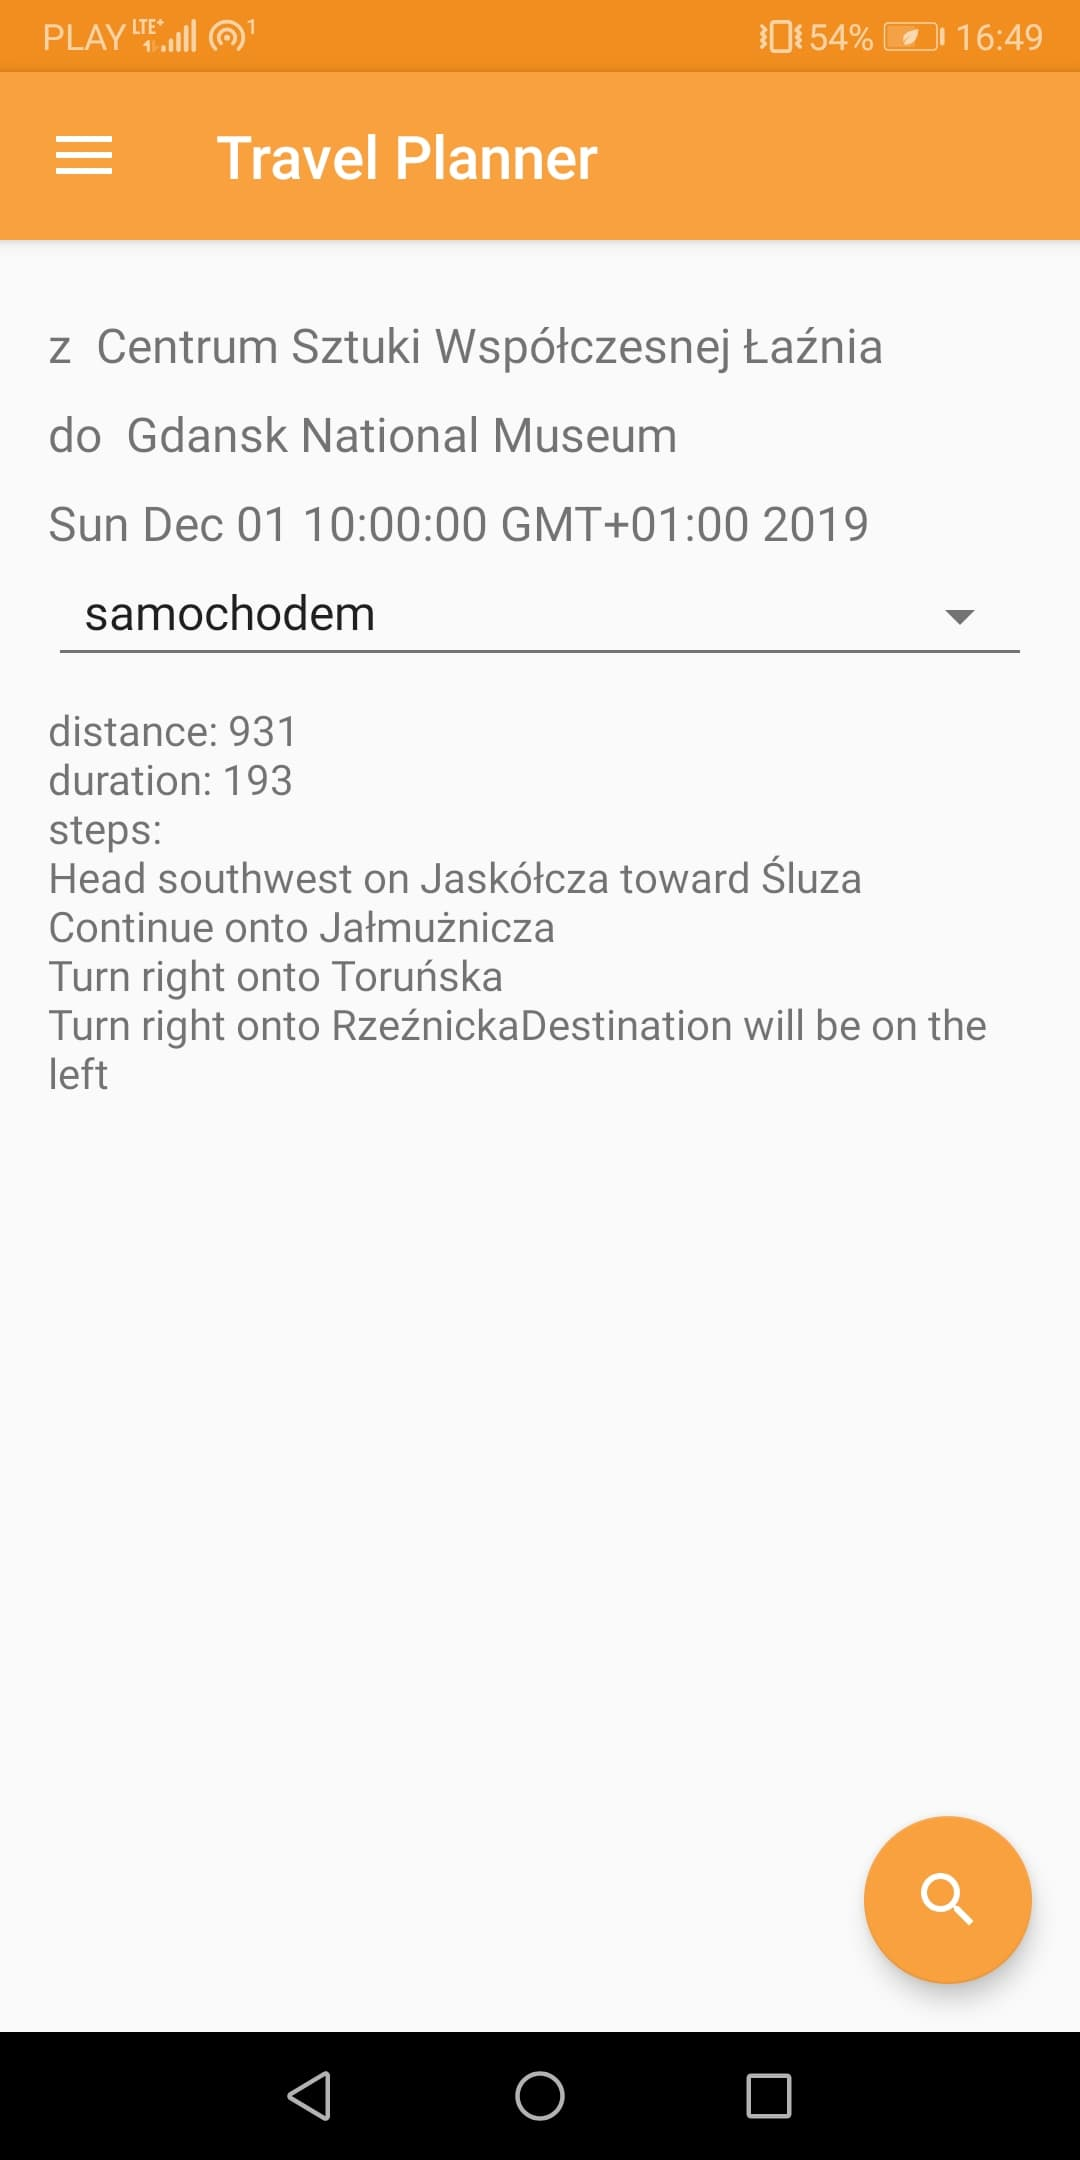
\includegraphics[width=0.4\textwidth]{transport2}}
\hfill\null

\caption{Wyszukiwanie transportu.}
\label{fig:podrecznik12}
\end{figure}
\FloatBarrier


\section{Czynności związane z elementami planu}
Aplikacja umożliwia wykonywanie kilku czynności związanych z poszczególnym elementem planu dnia. Oprócz możliwości odczytania szczegółowych informacji na jego temat można ocenić dane miejsce, oznaczyć plan jako ukończony oraz udostępnić go w medium społecznościowym.

\par Po kliknięciu na wybrany element pojawia się osobny widok zawierający dokładne informacje na temat wybranego miejsca (rys. 10.7a). Istnieje możliwość wystawienia oceny (rys. 10.7b).
Po przytrzymaniu palca na danym planu dnia pojawia się dymek z trzema opcjami do wyboru (rys. 10.8a).

\begin{figure}[h]

\centering
\null\hfill
\subfloat[Widok planu podróży.\label{fig:planElements}]{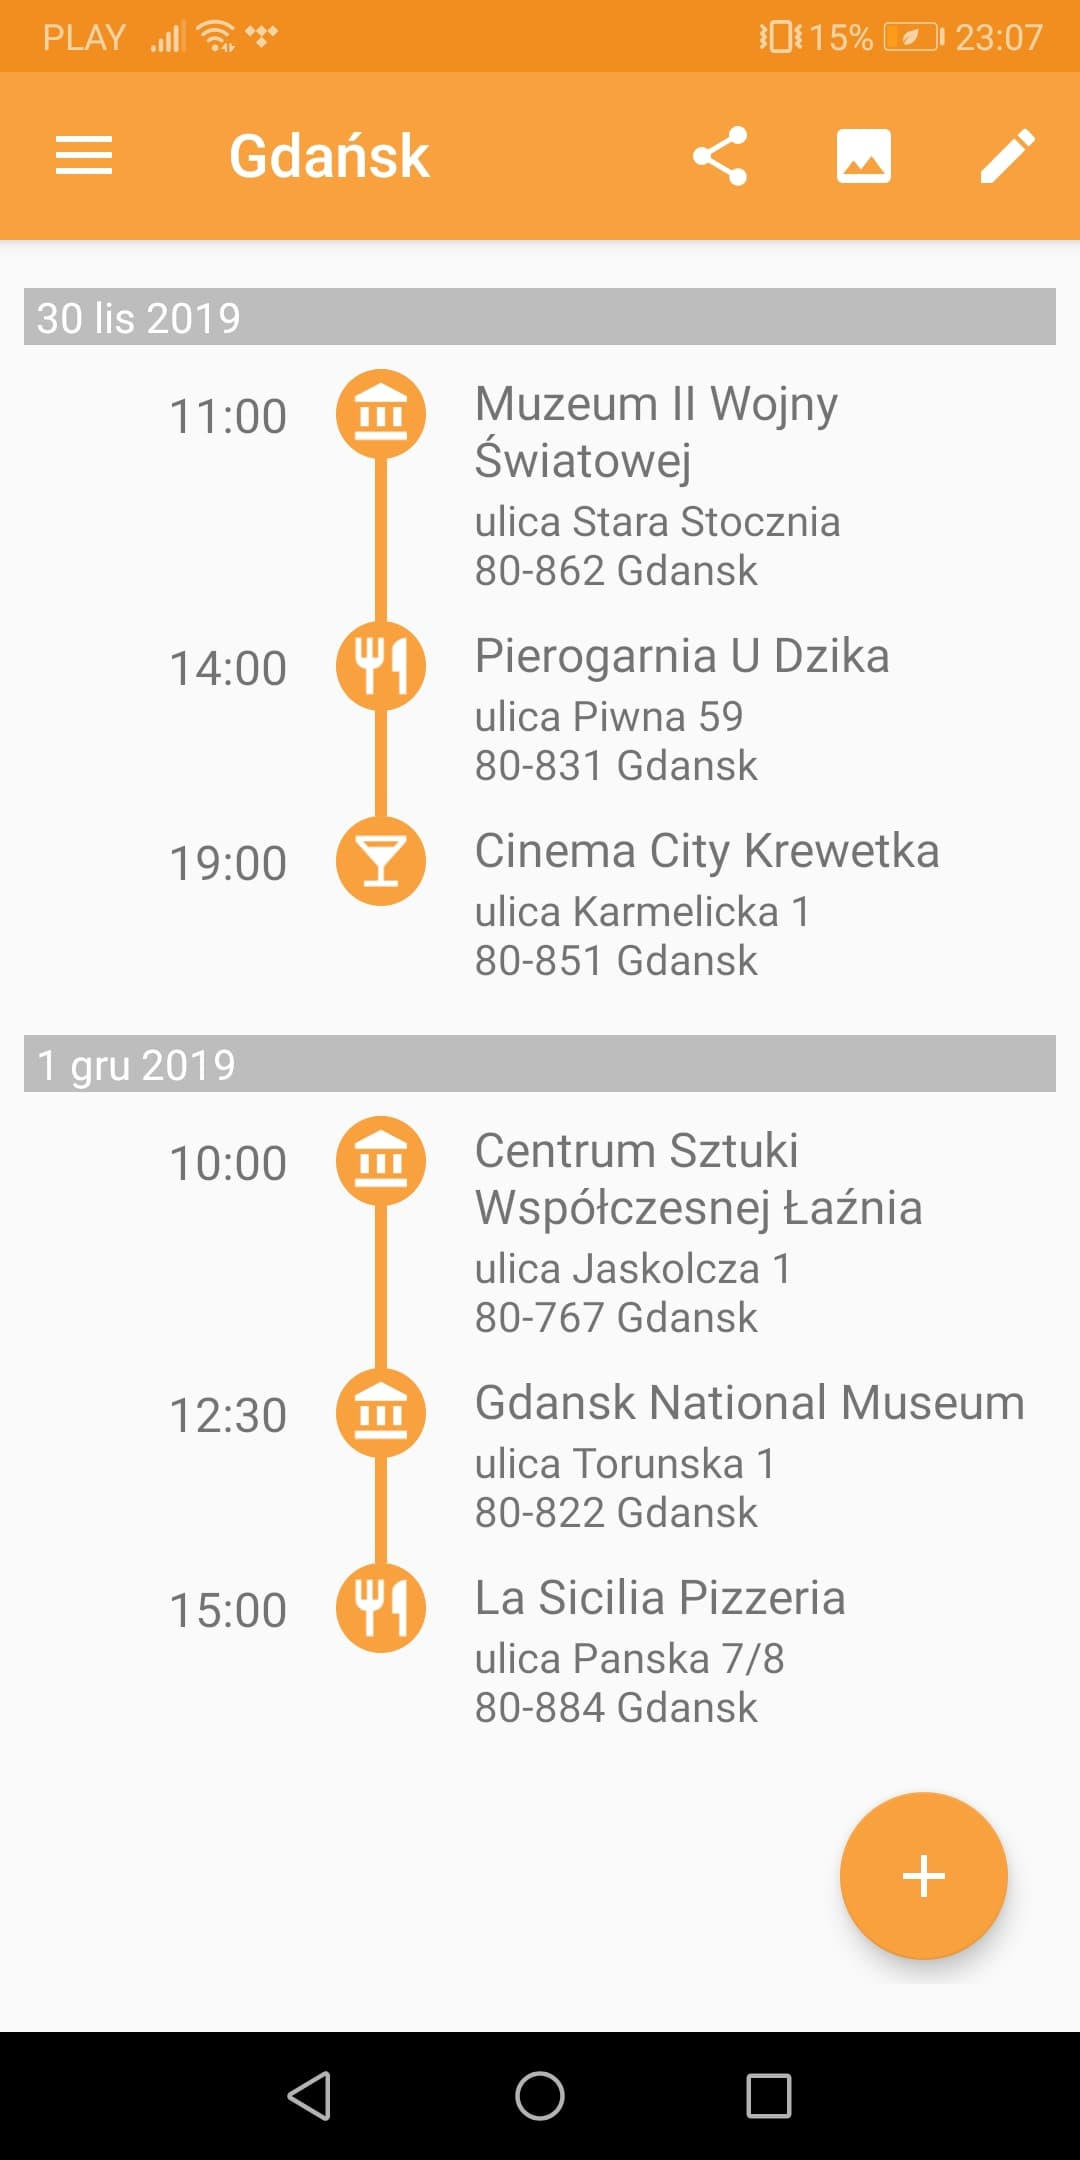
\includegraphics[width=0.4\textwidth]{planElements}}
\hfill
\subfloat[Ocenianie elementu planu.\label{fig:ratePlace2}]{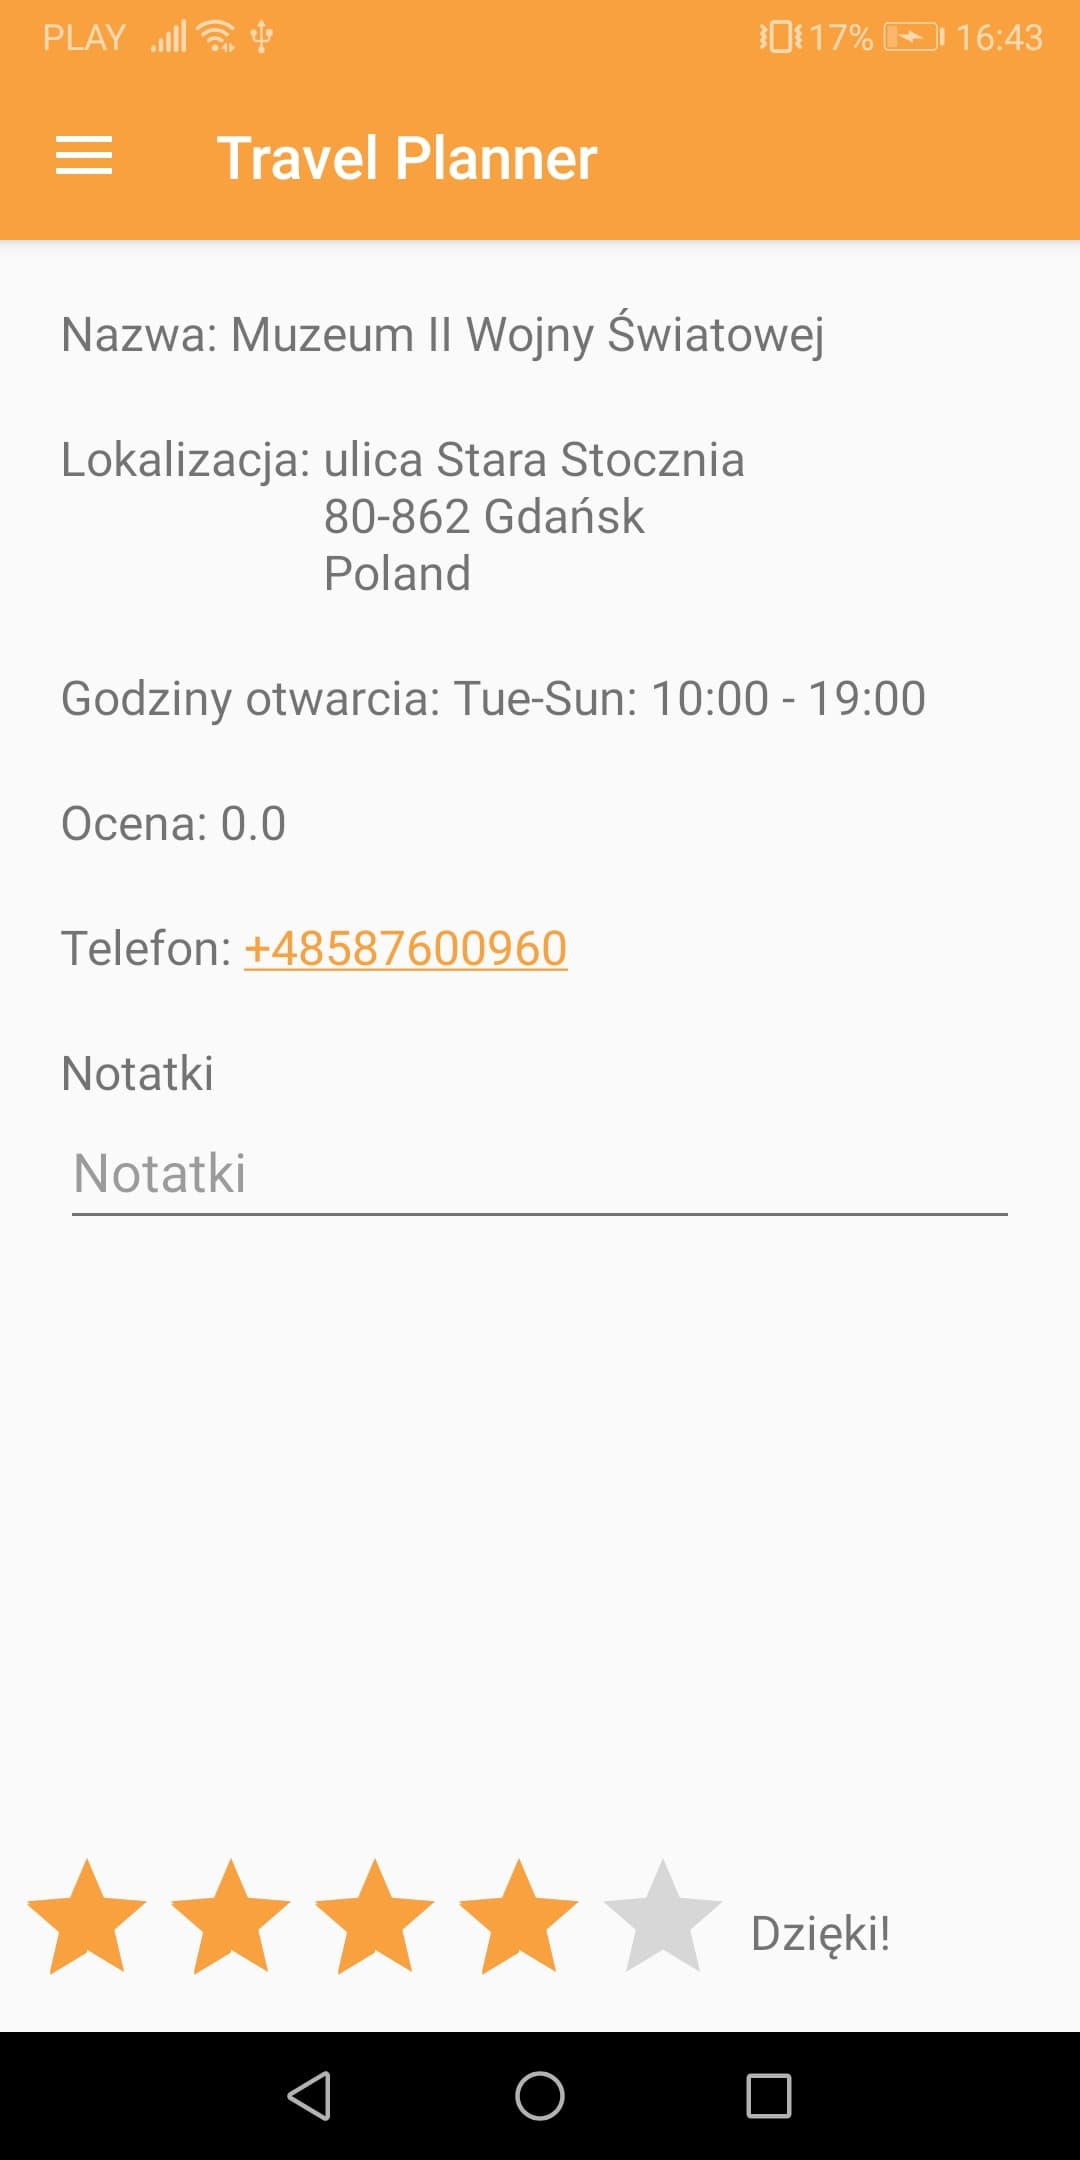
\includegraphics[width=0.4\textwidth]{ratePlace2}}
\hfill\null

\caption{Pojedyncza podróż.}
\label{fig:podrecznik4}
\end{figure}
\FloatBarrier

\begin{figure}[h]

\centering
\null\hfill
\subfloat[Opcje elementu planu.\label{fig:popUpMenu2}]{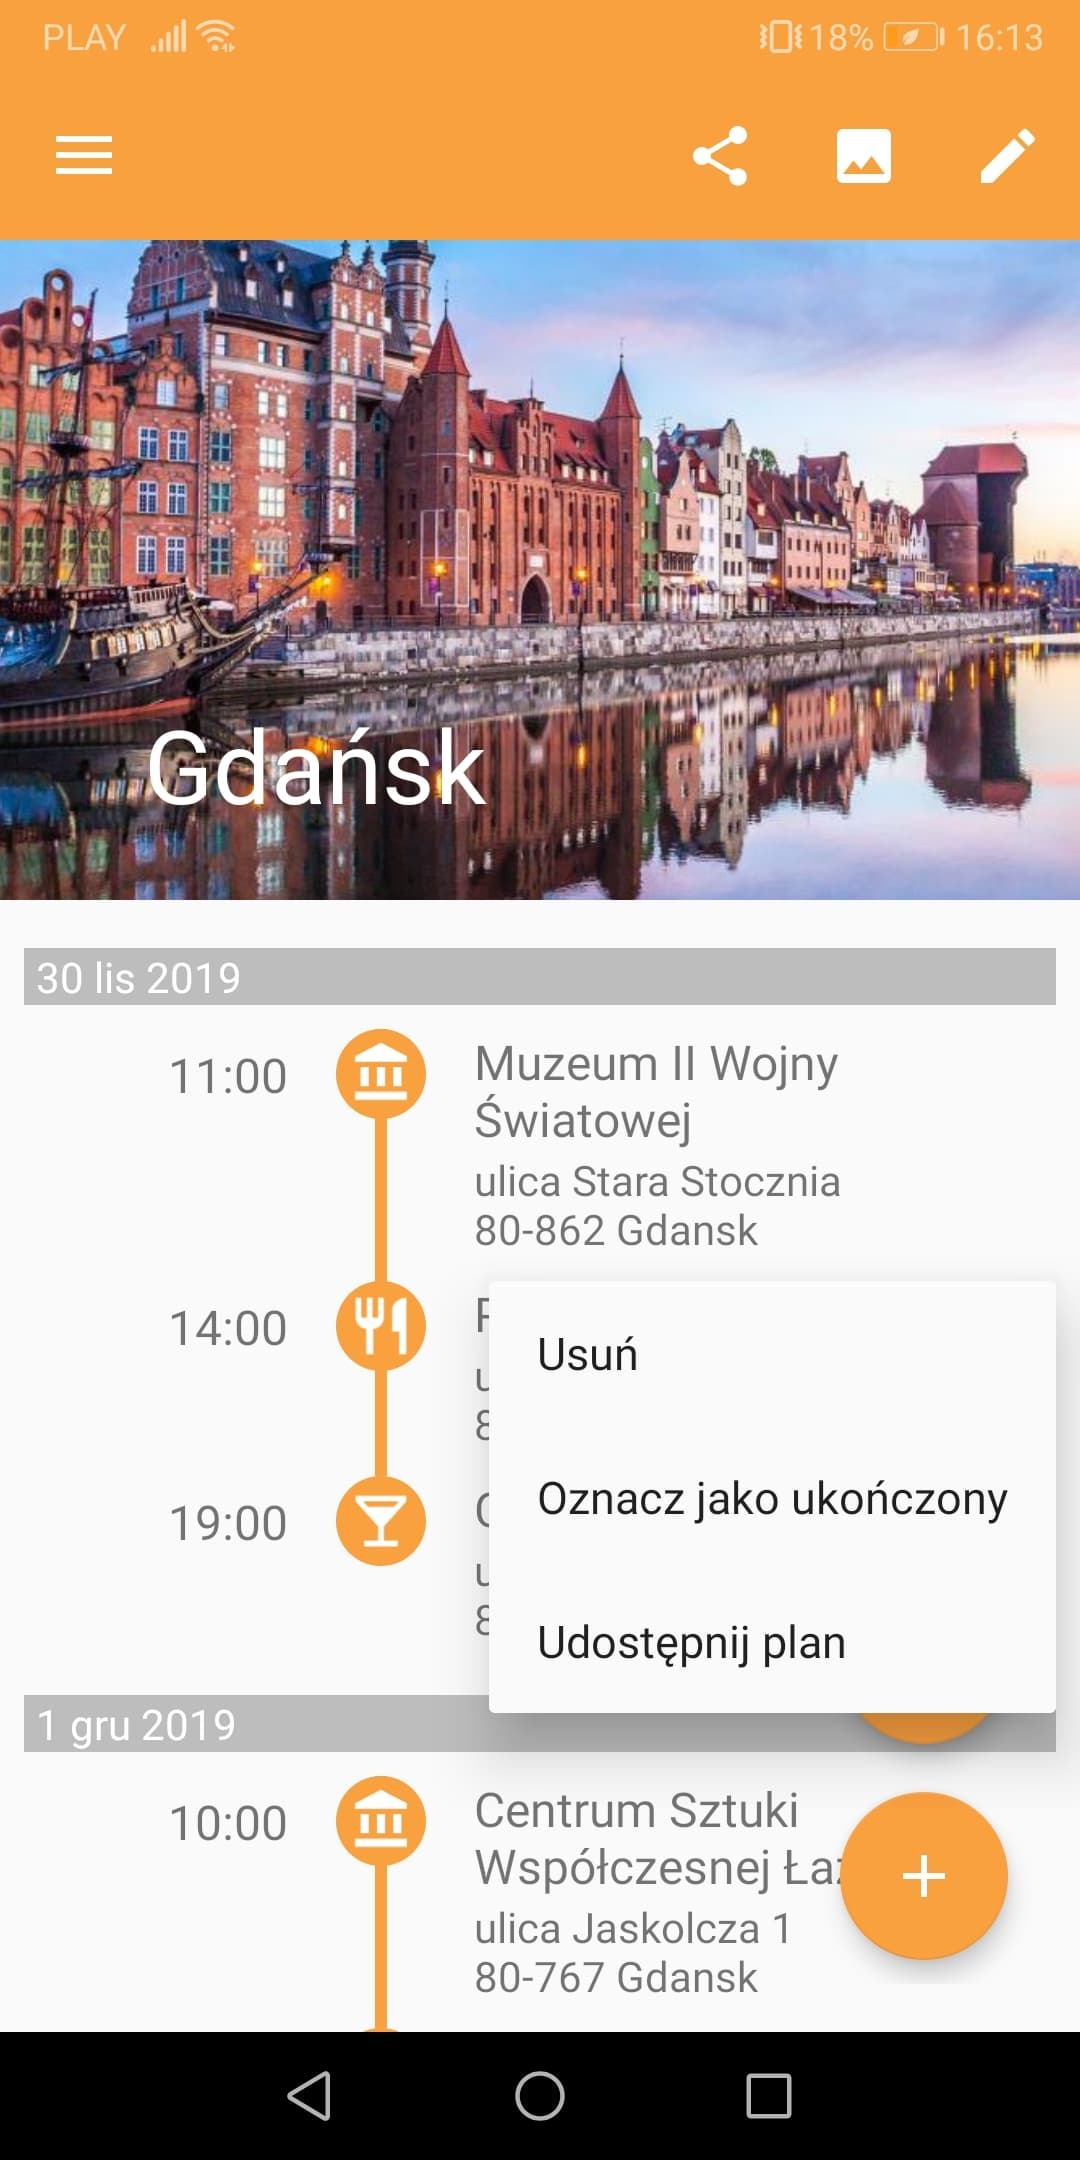
\includegraphics[width=0.32\textwidth]{popUpMenu2}}
\hfill
\subfloat[Tryb usuwania.\label{fig:deleteMode}]{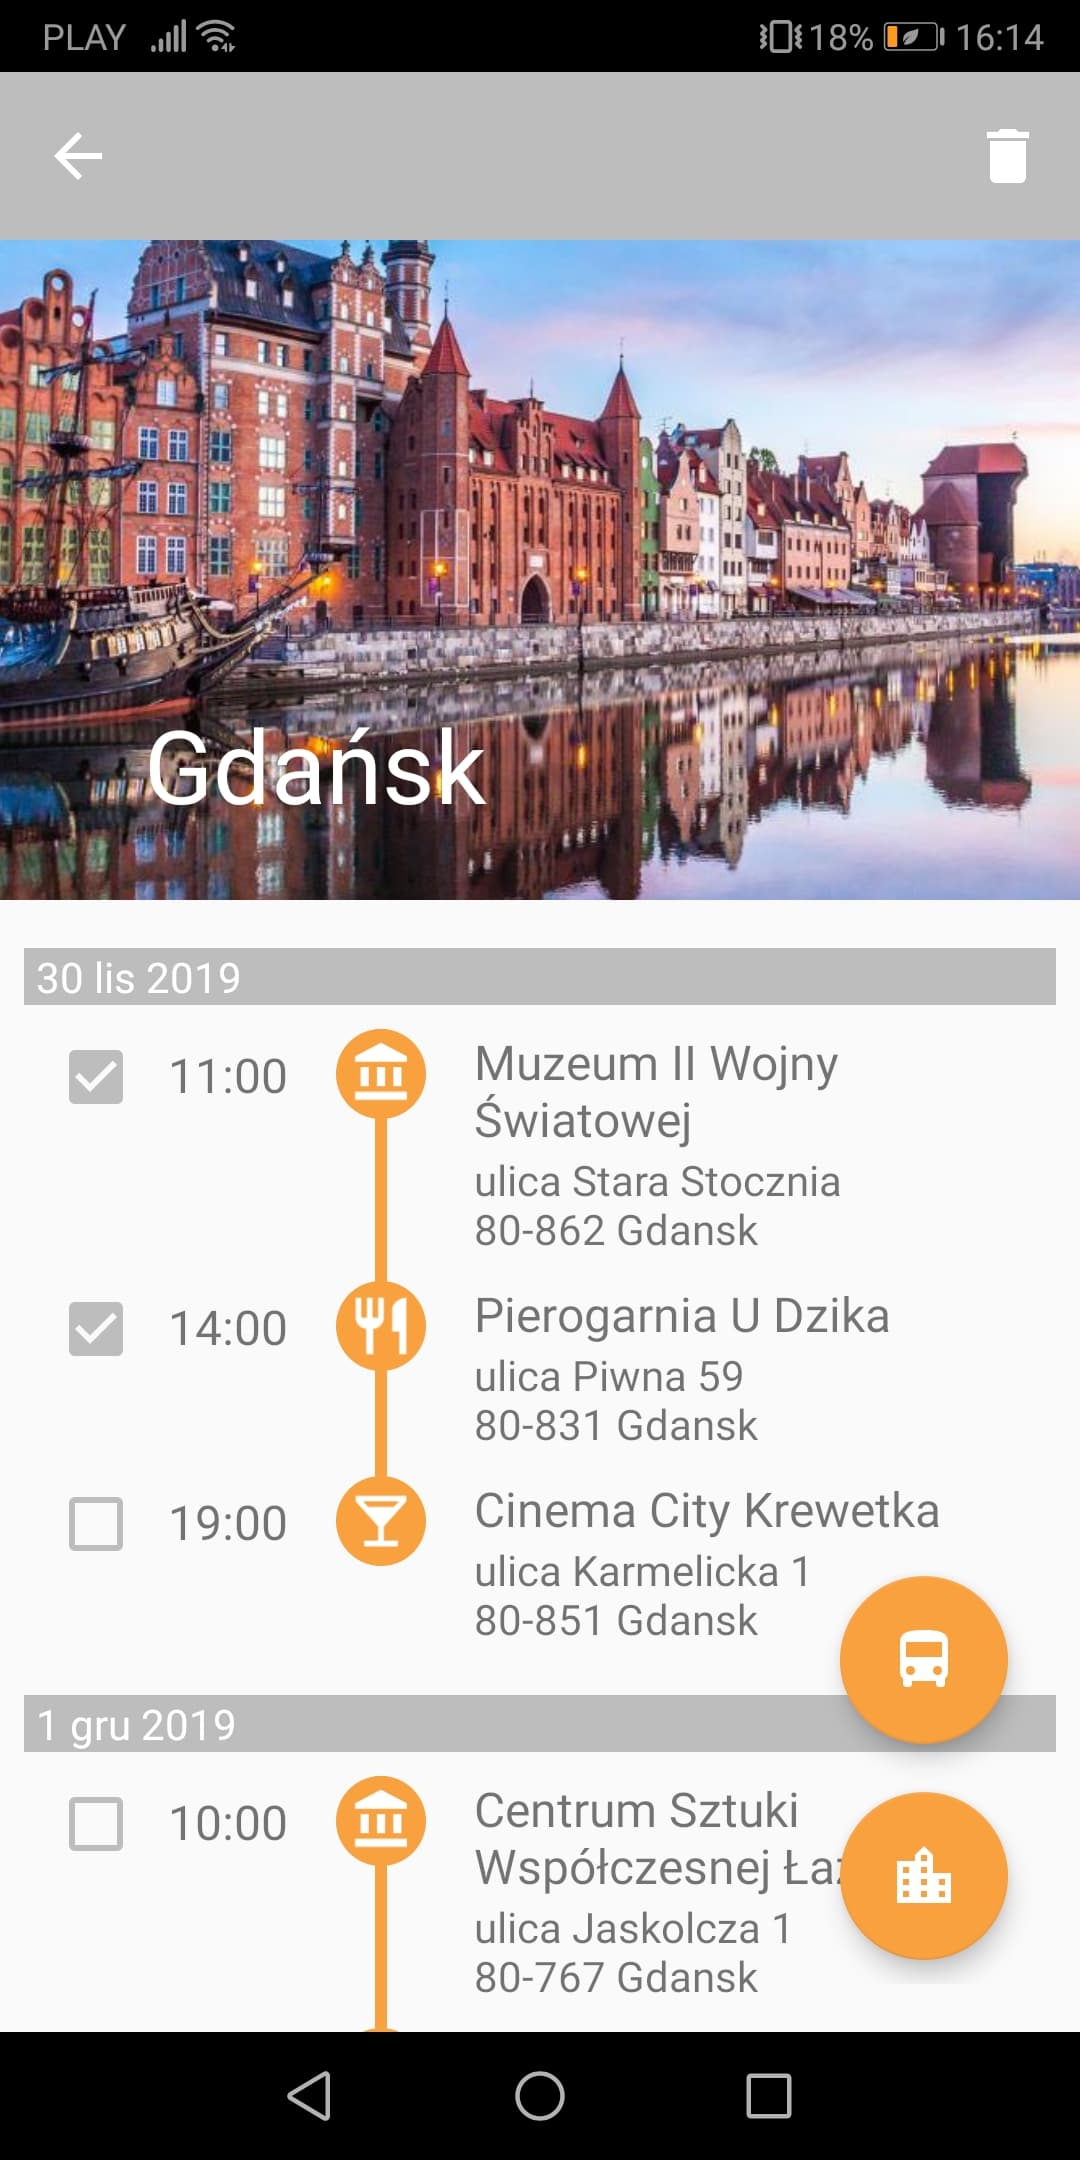
\includegraphics[width=0.32\textwidth]{deleteMode}}
\hfill
\subfloat[Manualna realizacja planu.\label{fig:popUpMenu}]{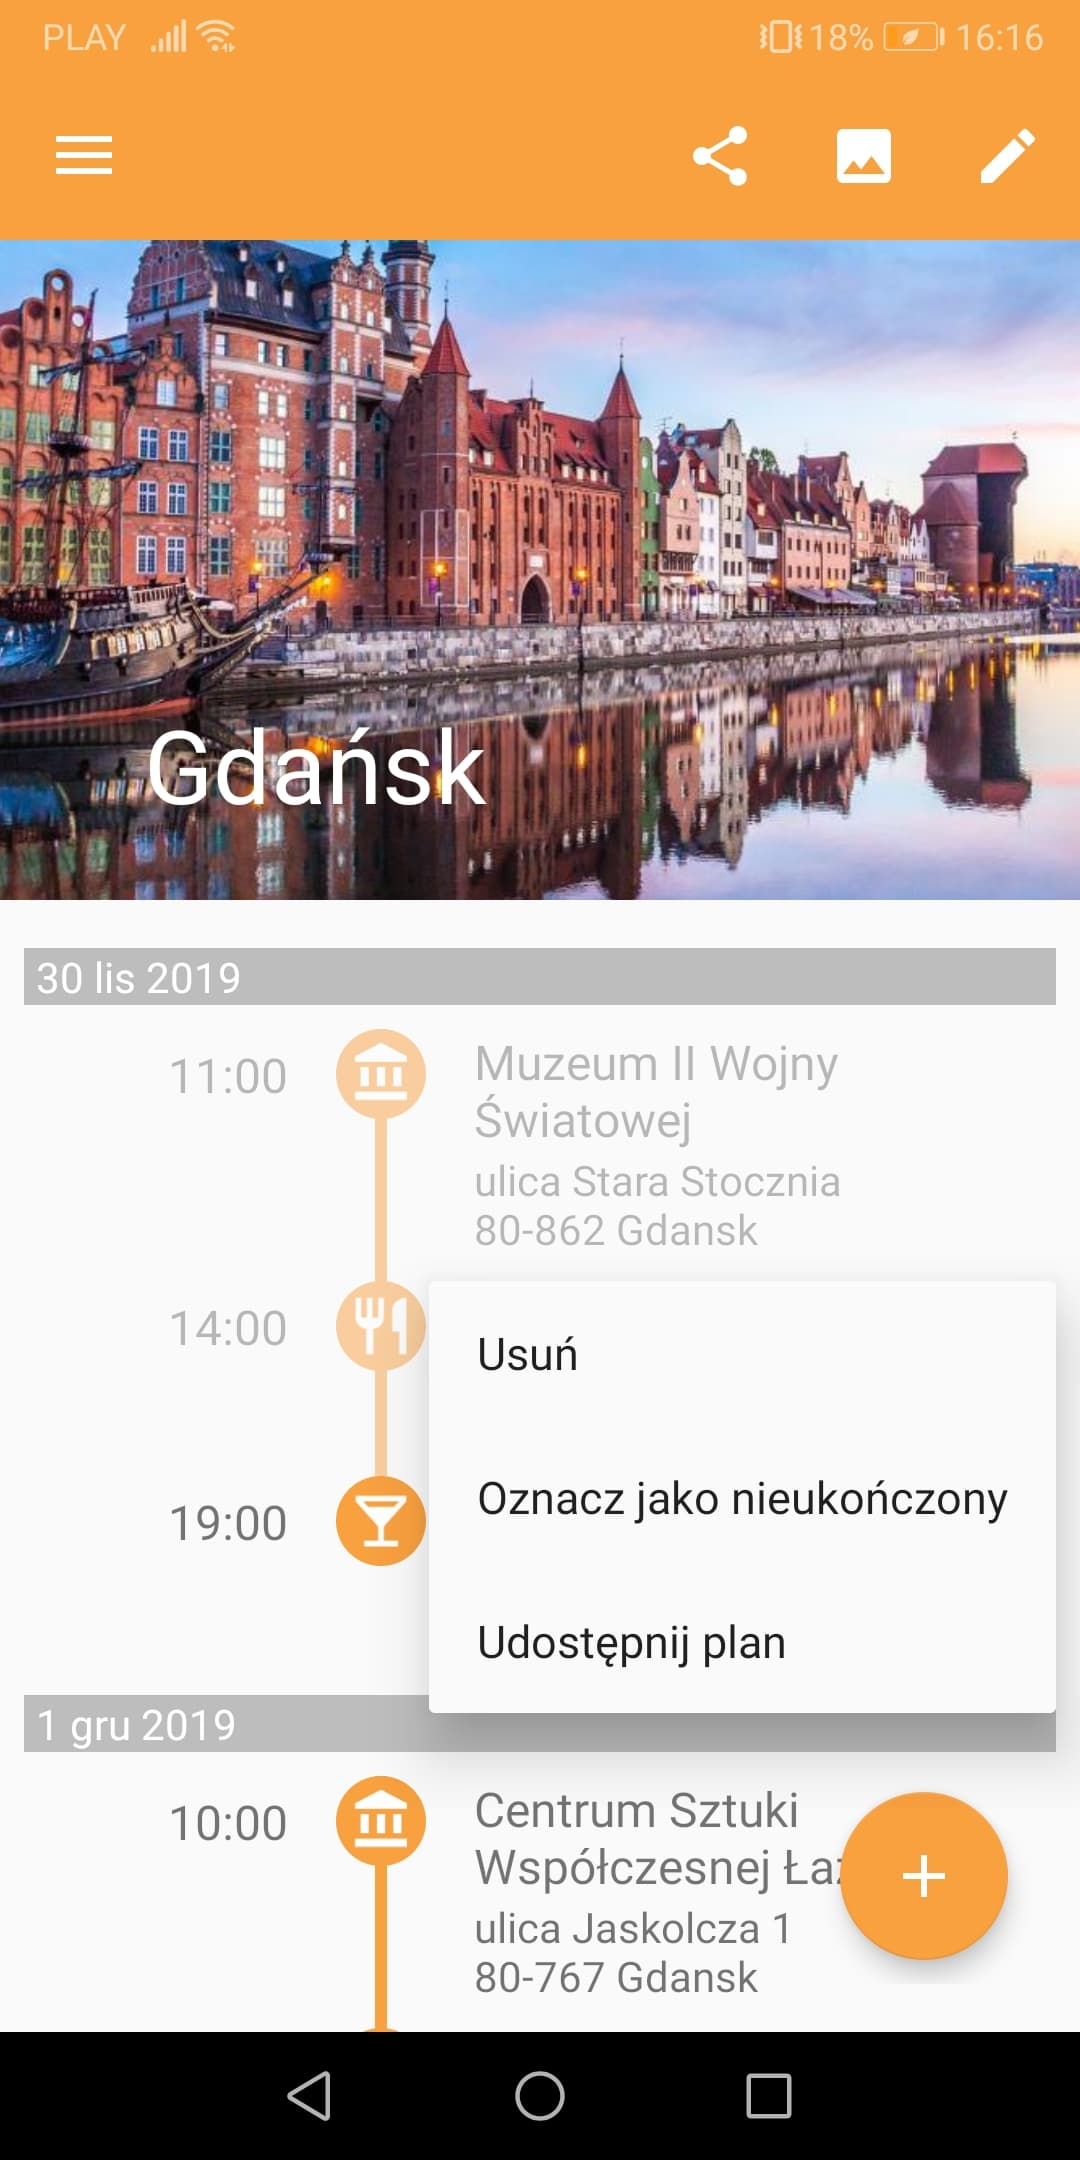
\includegraphics[width=0.32\textwidth]{popUpMenu}}
\hfill\null

\caption{Przytrzymanie elementu planu.}
\label{fig:podrecznik5}
\end{figure}
\FloatBarrier


Po wybraniu opcji \textit{Usuń} zostaje włączony tryb usuwania.
Jest on oznaczony jasnoszarym kolorem.
W celu usunięcia elementu należy:
\begin{enumerate}
\item Zaznaczyć wszystkie elementy, które mają być usunięte (rys. 10.8b).
\item Potwierdzić wykonanie czynności poprzez kliknięcie ikony kosza na śmieci.
\end{enumerate}
\textbf{UWAGA Przejście do trybu usuwania jest możliwe w każdym widoku zawierającym listę elementów. Przejście do niego jest wykonywane po dłuższym przytrzymaniu jednego z elementów.}



\par Manualna realizacja planu wygląda następująco (rys. 10.8c):
\begin{enumerate}
\item W przypadku ukończonego planu zawiera tekst \textit{Oznacz jako nieukończony}.
\item W przypadku nieukończonego planu zawiera tekst \textit{Oznacz plan jako ukończony}.
\end{enumerate}
Ukończone elementy planu dnia mają zmniejszoną intensywność kolorów.


\par Gdy użytkownik ma zainstalowaną aplikację Facebook posiada możliwość udostępnienia elementu planu na swojej \textit{tablicy}. W celu wykonania tej czynności należy:
\begin{enumerate}
\item Nacisnąć opcję \textit{Udostępnij}.
\item Napisać treść posta (rys. 10.9a).
\end{enumerate}
Domyślna tekst zawiera link do wybranego miejsca na mapie HERE (rys. 10.9b).

\begin{figure}[h]

\centering
\null\hfill
\subfloat[Udostępnianie posta.\label{fig:shareOnFacebook}]{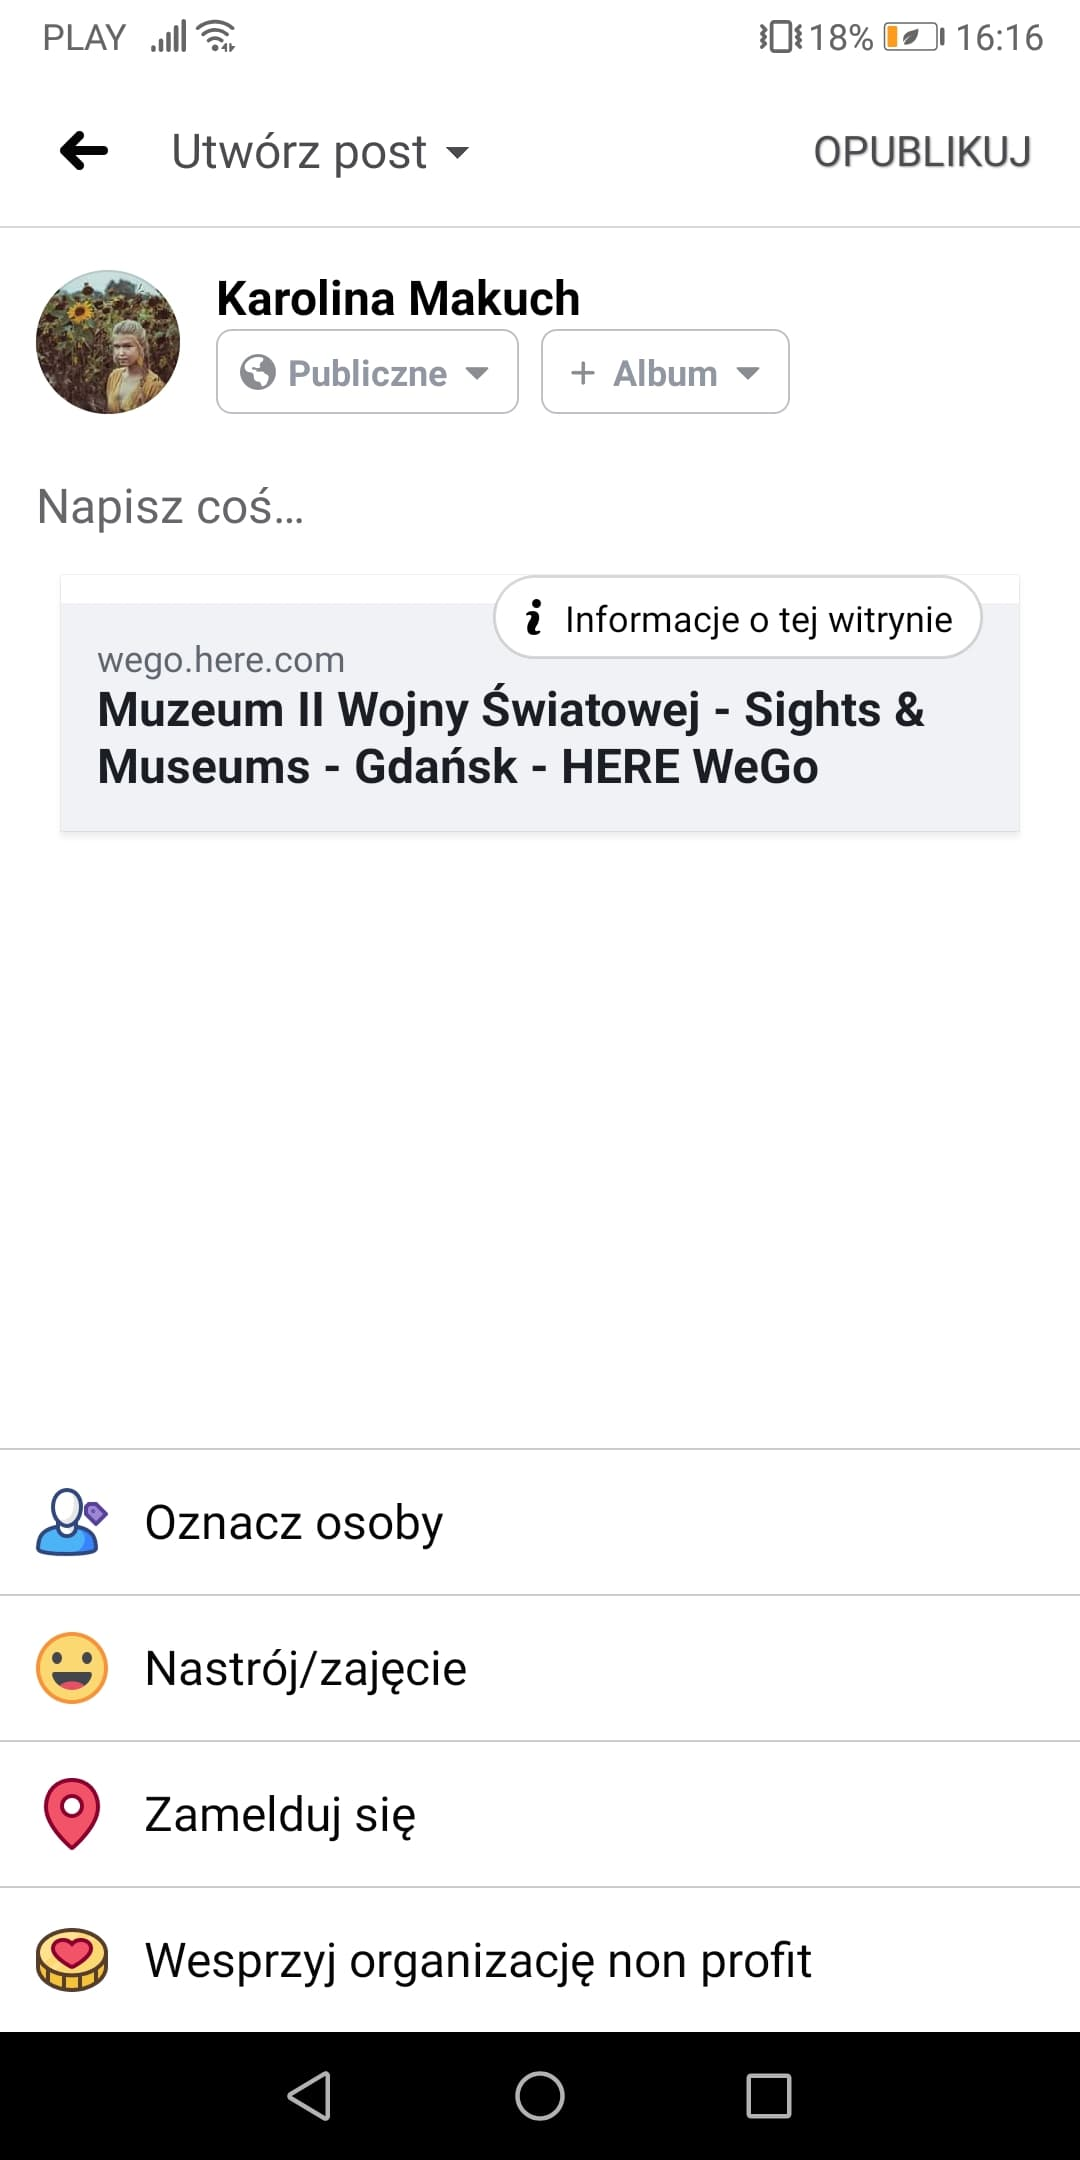
\includegraphics[width=0.4\textwidth]{shareOnFacebook}}
\hfill
\subfloat[Widok linku do map Here.\label{fig:hereMobile}]{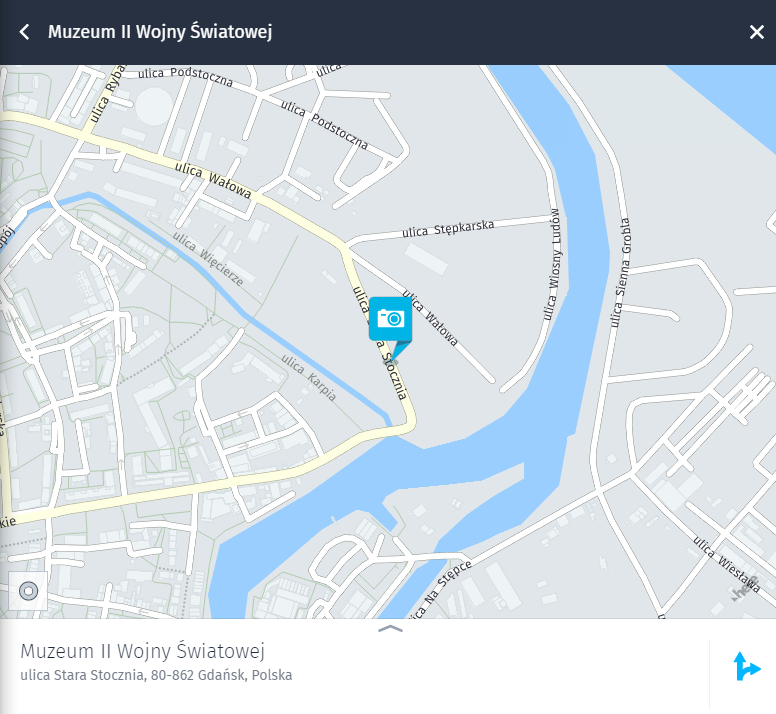
\includegraphics[width=0.55\textwidth]{hereMobile}}
\hfill\null

\caption{Udostępnianie elementu planu.}
\label{fig:podrecznik8}
\end{figure}
\FloatBarrier

\begin{figure}[h]

\centering
\null\hfill
\subfloat[Boczne menu.\label{fig:sideBar}]{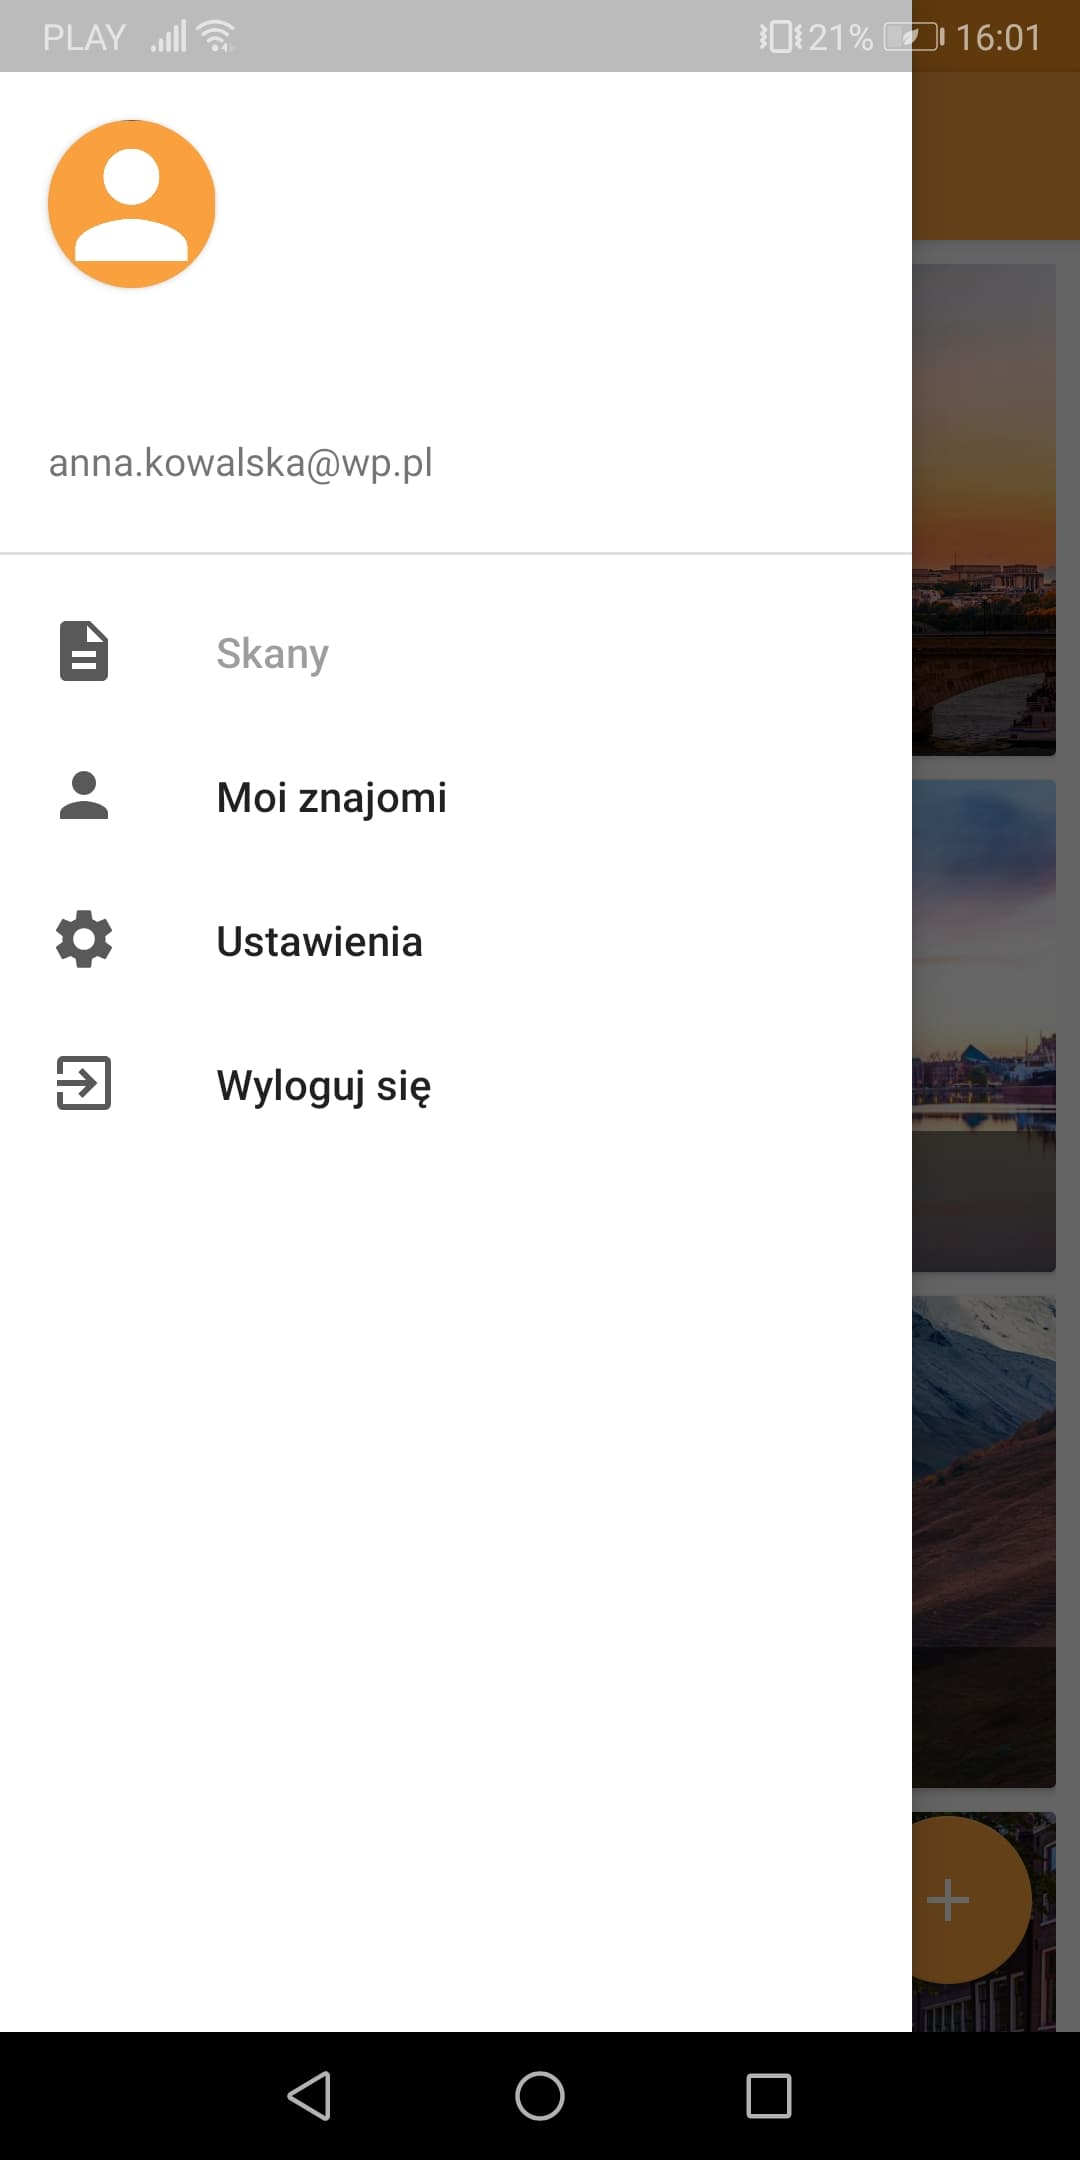
\includegraphics[width=0.4\textwidth]{sideBar}}
\hfill
\subfloat[Galeria skanów.\label{fig:scans}]{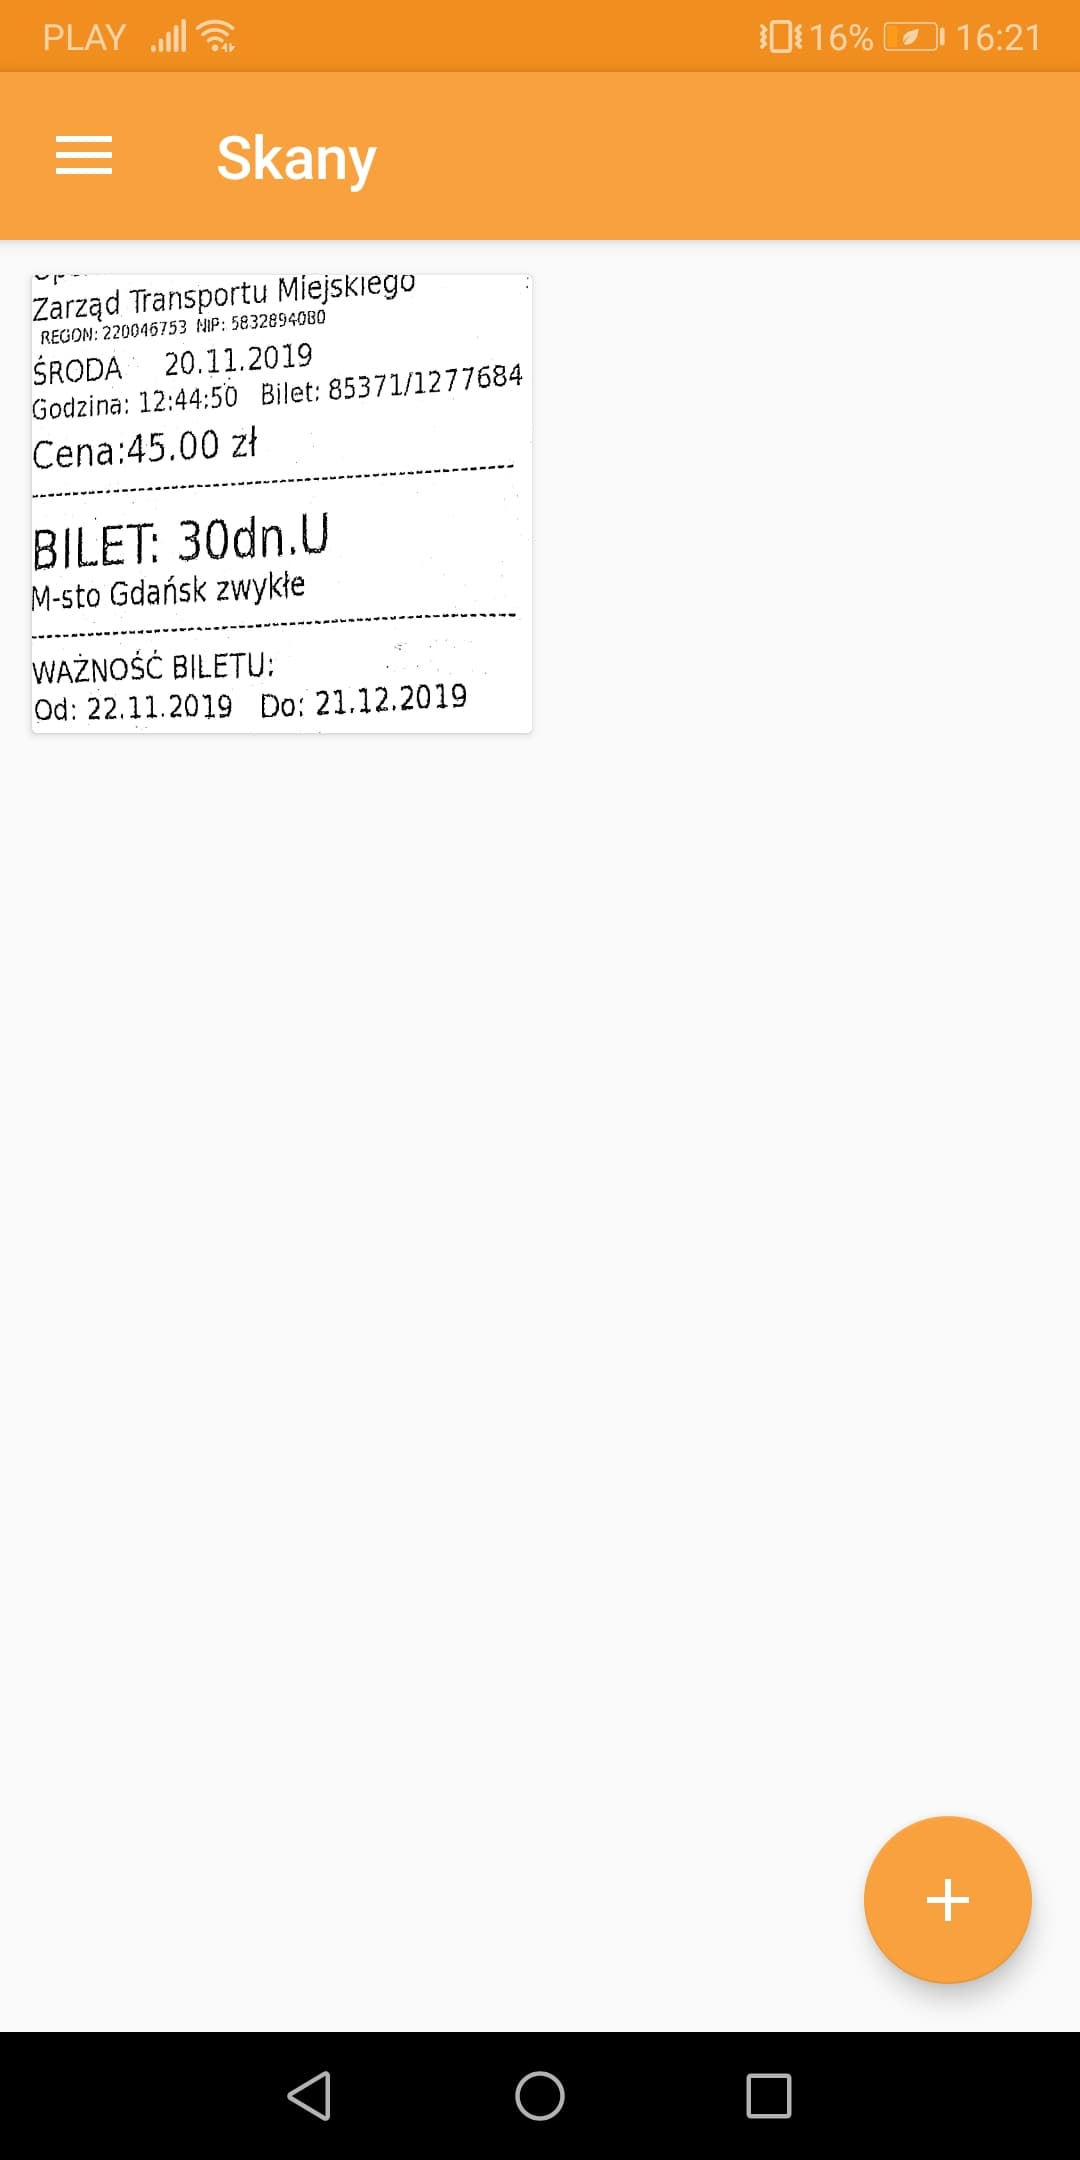
\includegraphics[width=0.4\textwidth]{scans}}
\hfill\null

\null\hfill
\subfloat[Wybór obszaru skanowania.\label{fig:sideBar}]{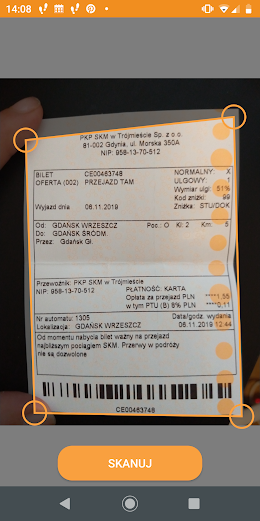
\includegraphics[width=0.4\textwidth]{scan1}}
\hfill
\subfloat[Obraz po przekształceniu.\label{fig:scan}]{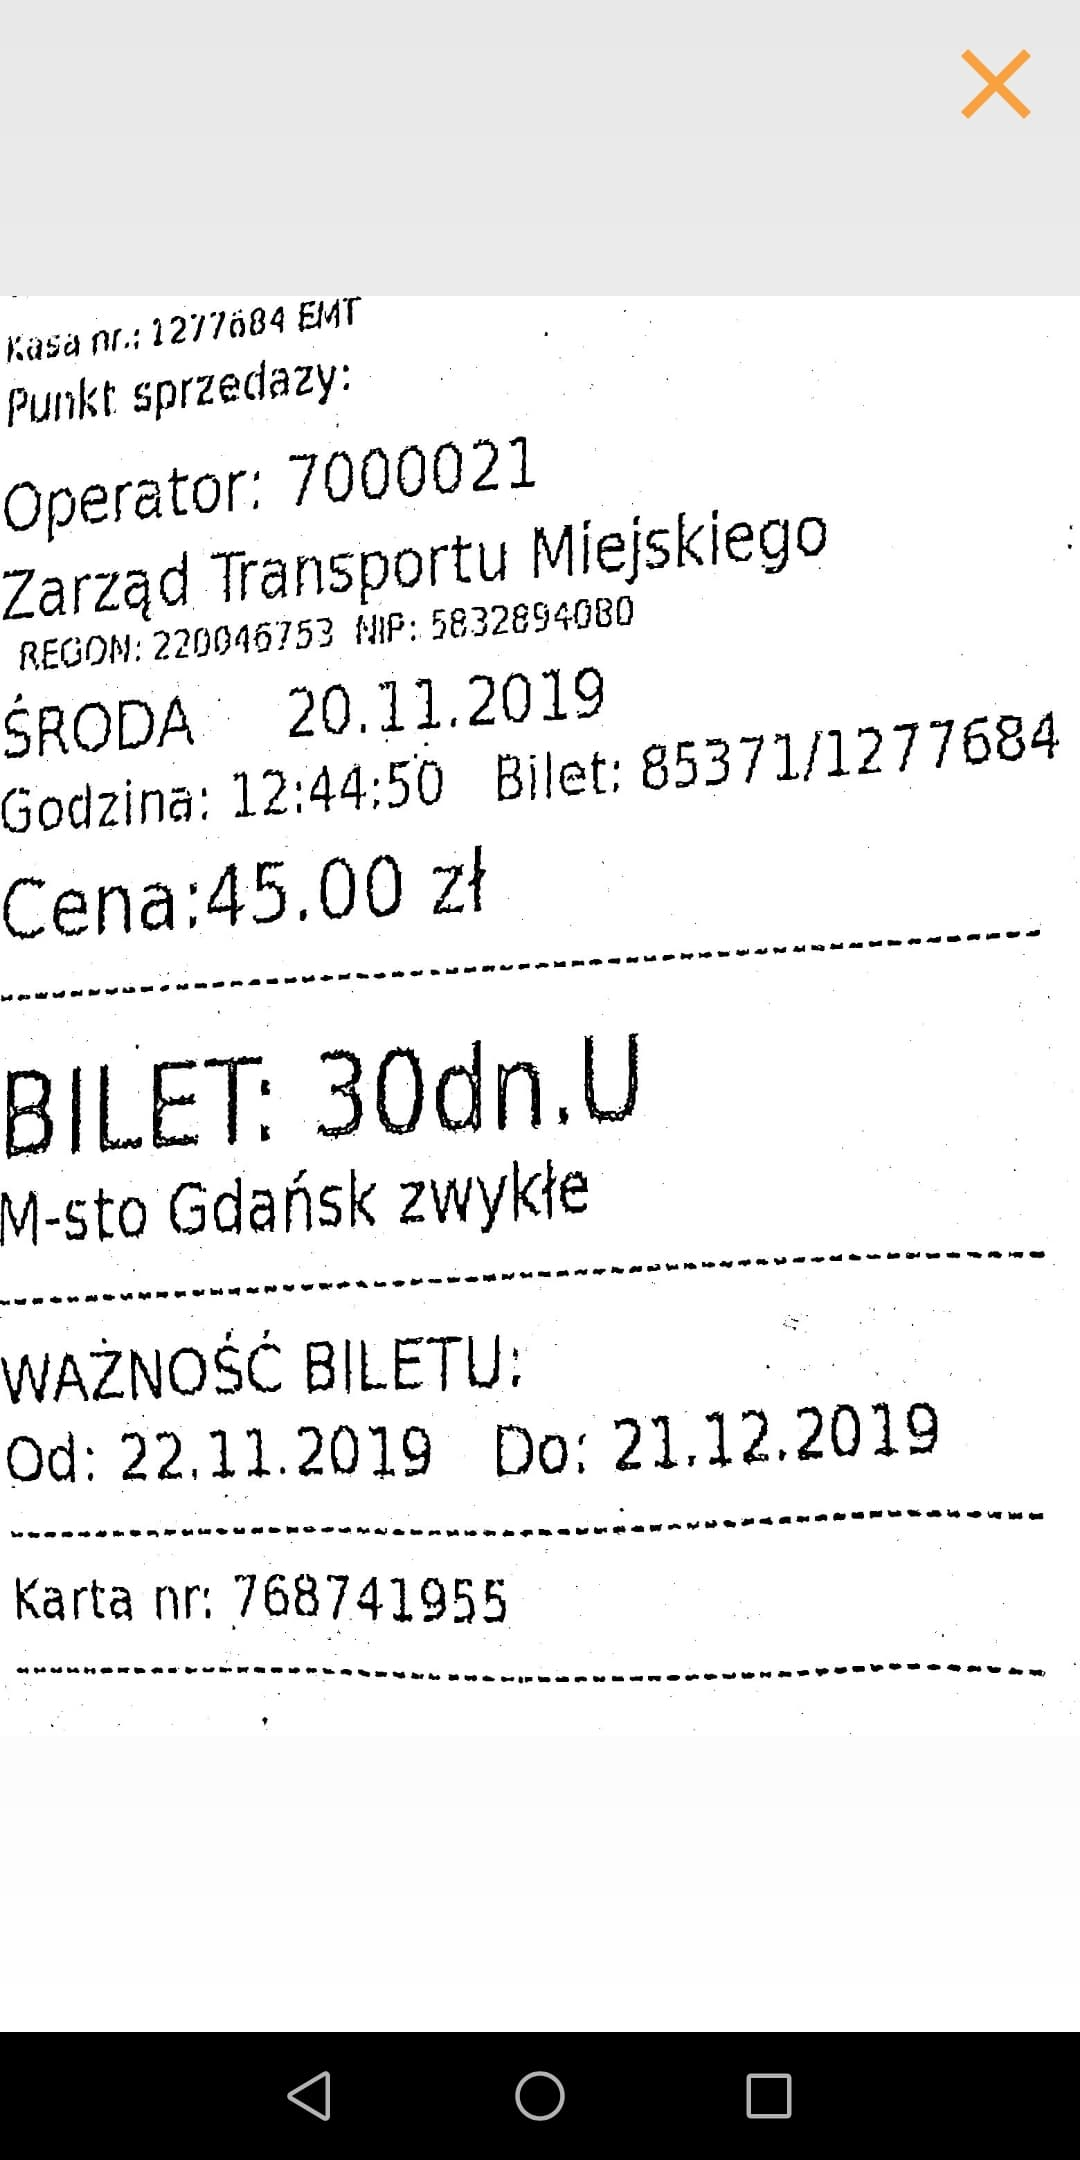
\includegraphics[width=0.4\textwidth]{scan}}
\hfill\null

\caption{Wykonanie skanu.}
\label{fig:podrecznik8}
\end{figure}
\FloatBarrier

\section{Skanowanie dokumentów}
Użytkownik posiadający plan podróży ma możliwość dodania skanu – czarno-białego zdjęcia po progowaniu.
W celu przechowania dokumentu w aplikacji należy:
\begin{enumerate}
\item Kliknąć na symbol szuflady nawigacji (ang. hamburger).
\item W bocznym menu wybrać \textit{Skany} (rys. 10.10a).
\item Nacisnąć przycisk zawierający symbol \textit{+} (rys. 10.10b).
\item Wyrazić zgodę na dostęp do aparatu.
\item Wykonać zdjęcie dokumentu.
\item Wybrać interesujący obszar (dowolny czworokąt) (rys. 10.10c).
\item Zaakceptować przekształcenie obrazu klikając przycisk \textit{Skanuj} (rys. 10.10d).
\item Miniatura skanu pojawi się w galerii.
\end{enumerate}

\section{Znajomi}
Chcąc udostępnić innemu użytkownikowi podróży należy go wcześniej dodać do znajomych. Można to zrobić w następujących krokach:
\begin{enumerate}
\item Kliknąć na symbol szuflady nawigacji (and. hamburger menu).
\item W bocznym menu wybrać \textit{Znajomi}.
\item Wpisać w wyszukiwarce adres mailowy danego użytkownika.
\item Wybrać odpowiedni mail z podpowiedzi (rys.10. 11a).
\item Potwierdzić chęć dodania do znajomych, poprzez kliknięcie \textit{OK} (rys. 10.11b).
\item W przypadku prawidłowego wykonania czynności użytkownik zostanie automatycznie dodany do listy znajomych oraz pojawi się odpowiednie powiadomienie (rys 10.11c).
\end{enumerate}

\begin{figure}[h]

\null\hfill
\subfloat[Wyszukiwanie znajomych.\label{fig:friends1}]{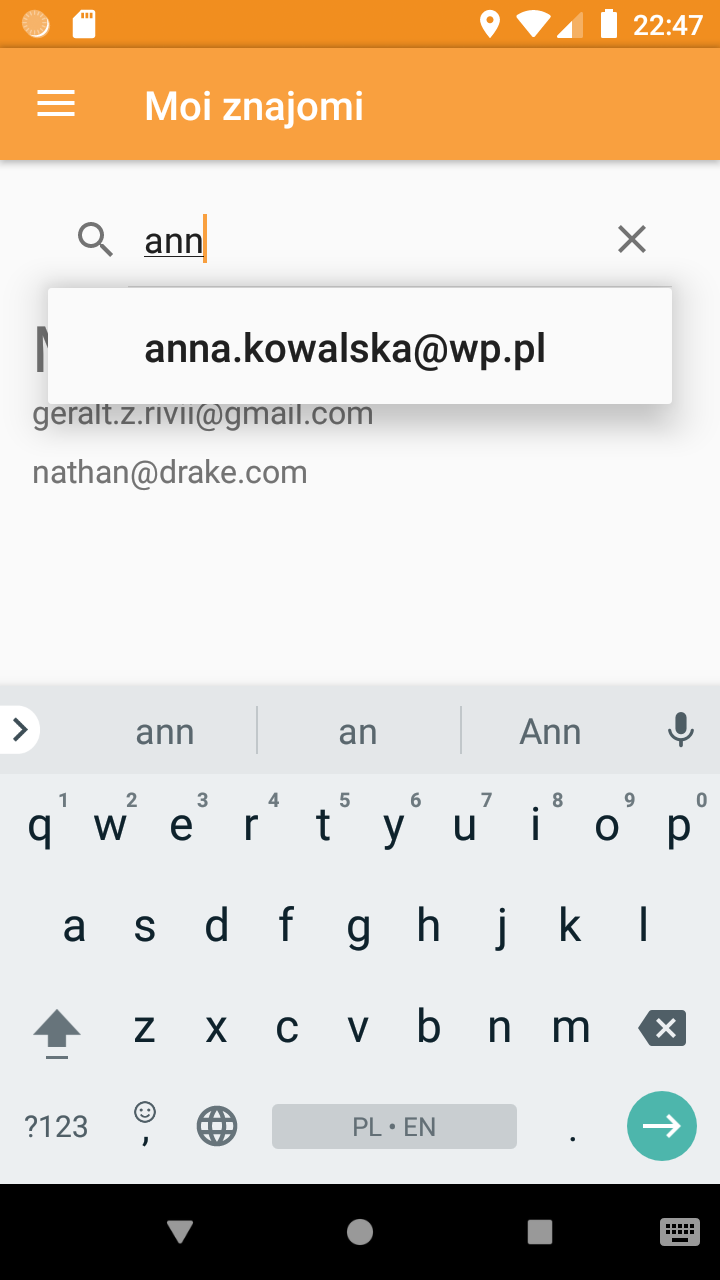
\includegraphics[width=0.32\textwidth]{friends1}}
\hfill
\subfloat[Potwierdzenie decyzji.\label{fig:friends2}]{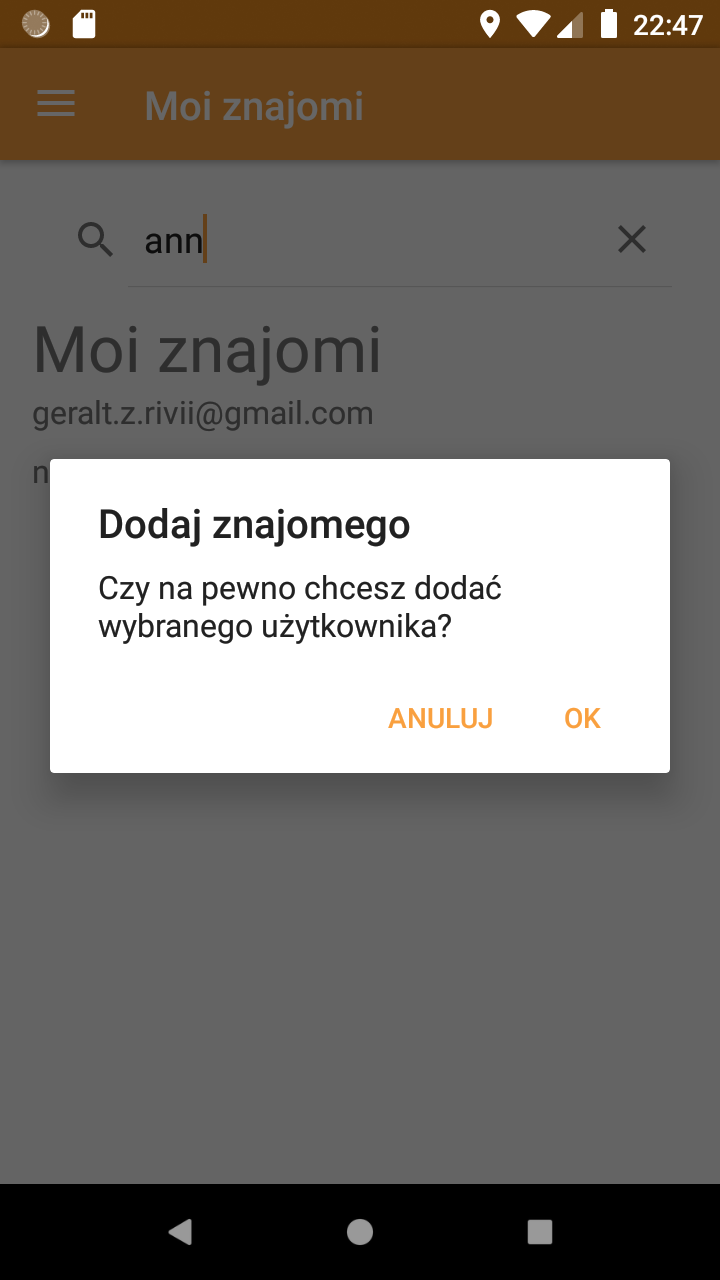
\includegraphics[width=0.32\textwidth]{friends2}}
\hfill
\subfloat[Wynik.\label{fig:friends3}]{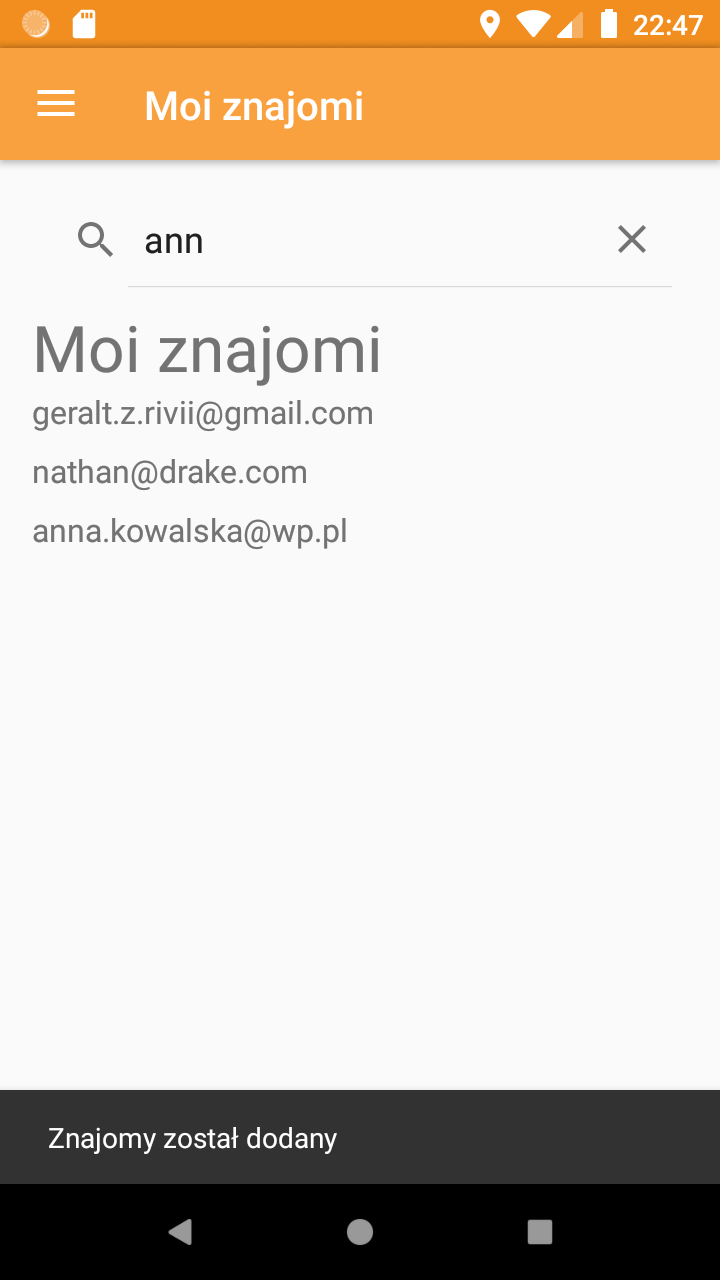
\includegraphics[width=0.32\textwidth]{friends3}}
\hfill\null

\caption{Dodawanie znajomych.}
\label{fig:podrecznik9}
\end{figure}
\FloatBarrier


\section{Rekomendacja miejsc}
Bazując na opiniach innych użytkowników aplikacja wyświetla listę polecanych miejsc. W trakcie korzystania z aplikacji użytkownik:
\begin{enumerate}
\item Dostaje powiadomienie o znalezieniu miejsc wartych jego uwagi.
\item Klika na powiadomienie od aplikacji (rys. 10.12a).
\item Zostaje przekierowany do aplikacji z wyświetlonym oknem zawierającym listę rekomendowanych miejsc (rys. 10.12b).
\end{enumerate}
\begin{figure}[h]

\centering
\null\hfill
\subfloat[Powiadomienie aplikacji.\label{fig:recomendation1}]{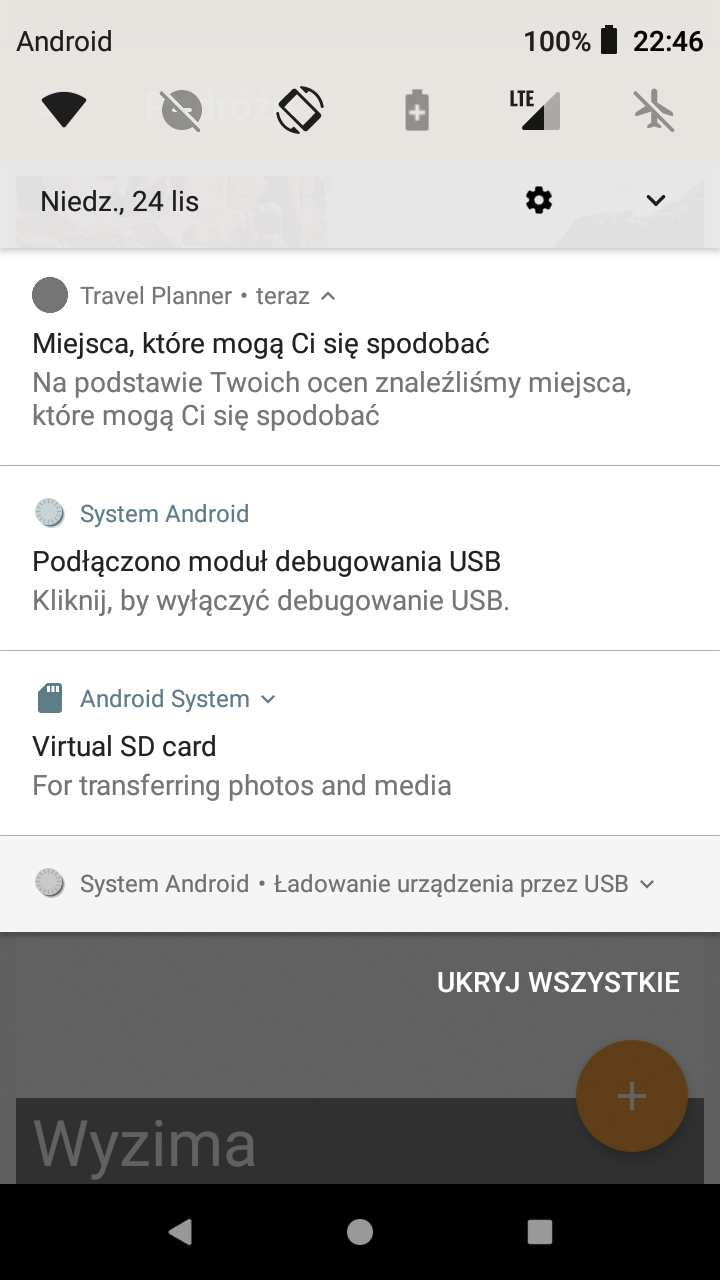
\includegraphics[width=0.4\textwidth]{recomendation1}}
\hfill
\subfloat[Lista miejsc wartych uwagi.\label{fig:recomendation2}]{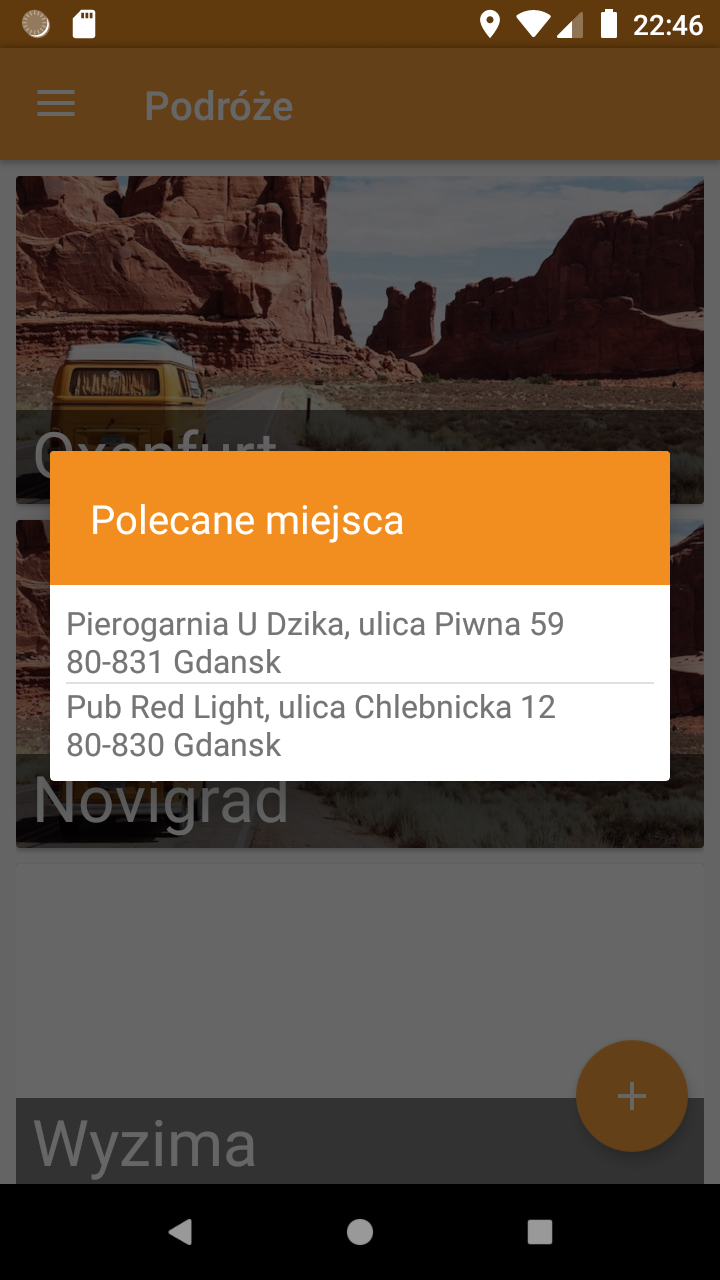
\includegraphics[width=0.4\textwidth]{recomendation2}}
\hfill\null

\caption{Rekomendacja atrakcji.}
\label{fig:podrecznik11}
\end{figure}
\FloatBarrier